\documentclass[a4paper,11pt]{book}
%\documentclass[a4paper,twoside,11pt,titlepage]{book}
\raggedbottom
\usepackage{listings}
\usepackage[utf8]{inputenc}
\usepackage{pmboxdraw}
\usepackage[spanish]{babel}
\usepackage{xspace}

% \usepackage[style=list, number=none]{glossary} %
\usepackage{titlesec}
%\usepackage{pailatino}

\decimalpoint
\usepackage{dcolumn}
\newcolumntype{.}{D{.}{\esperiod}{-1}}
\makeatletter
\addto\shorthandsspanish{\let\esperiod\es@period@code}
\makeatother


\usepackage[chapter]{algorithm}
\usepackage{algpseudocode}
\RequirePackage{verbatim}
%\RequirePackage[Glenn]{fncychap}
\usepackage{fancyhdr}
\usepackage{graphicx}
\usepackage{tikz}
\usetikzlibrary{positioning}
\usetikzlibrary{babel}
\usetikzlibrary{arrows.meta}
\usetikzlibrary{calc}
\usepackage{float}
\usepackage{afterpage}

\usepackage{longtable}
\usepackage{enumitem}
\usepackage{tabularx}
\usepackage{subcaption}

\makeatletter
\newcommand{\twodigits}[1]{\expandafter\@twodigits\csname c@#1\endcsname}
\newcommand{\@twodigits}[1]{\ifnum#1<10 0\fi\number#1}
\makeatother
\AddEnumerateCounter*{\twodigits}{\@twodigits}{99}

\usepackage[hidelinks]{hyperref} %referencia

% ********************************************************************
% Re-usable information
% ********************************************************************
\newcommand{\myTitle}{Desarrollo de un sistema inteligente para Onitama con visión por computador\xspace}
\newcommand{\mySubTitle}{Reconstrucción automática del estado de una partida física y selección de jugadas mediante Minimax con poda alfa-beta\xspace}
\newcommand{\myDegree}{Grado en Ingeniería Informática\xspace}
\newcommand{\myName}{Mariano Aguilar Olmo\xspace}
\newcommand{\myProf}{Salvador García López\xspace}
\newcommand{\myFaculty}{Escuela Técnica Superior de Ingenierías Informática y de
Telecomunicación\xspace}
\newcommand{\myFacultyShort}{E.T.S. de Ingenierías Informática y de
Telecomunicación\xspace}
\newcommand{\myDepartment}{Departamento de Ciencias de la Computación e Inteligencia Artificial\xspace}
\newcommand{\myUni}{\protect{Universidad de Granada}\xspace}
\newcommand{\myLocation}{Granada\xspace}
\newcommand{\myTime}{\today\xspace}
\newcommand{\myVersion}{Version 0.1\xspace}


\hypersetup{
pdfauthor = {\myName (marianoaguilar@correo.ugr.es)},
pdftitle = {\myTitle},
pdfsubject = {},
pdfkeywords = {palabra_clave1, palabra_clave2, palabra_clave3, ...},
pdfcreator = {LaTeX con el paquete ....},
pdfproducer = {pdflatex}
}

%\hyphenation{}


%\usepackage{doxygen/doxygen}
%\usepackage{pdfpages}
\usepackage{url}
\usepackage{colortbl,longtable}
\usepackage[stable]{footmisc}
%\usepackage{index}

%\makeindex
%\usepackage[style=long, cols=2,border=plain,toc=true,number=none]{glossary}
% \makeglossary

% Definición de comandos que me son tiles:
%\renewcommand{\indexname}{Índice alfabético}
%\renewcommand{\glossaryname}{Glosario}

\pagestyle{fancy}
\fancyhf{}
\fancyhead[LO]{\leftmark}
\fancyhead[RE]{\rightmark}
\fancyhead[RO,LE]{\textbf{\thepage}}
\renewcommand{\chaptermark}[1]{\markboth{\textbf{#1}}{}}
\renewcommand{\sectionmark}[1]{\markright{\textbf{\thesection. #1}}}

\setlength{\headheight}{1.5\headheight}

\newcommand{\HRule}{\rule{\linewidth}{0.5mm}}
%Definimos los tipos teorema, ejemplo y definición podremos usar estos tipos
%simplemente poniendo \begin{teorema} \end{teorema} ...
\newtheorem{teorema}{Teorema}[chapter]
\newtheorem{ejemplo}{Ejemplo}[chapter]
\newtheorem{definicion}{Definición}[chapter]

\definecolor{gray97}{gray}{.97}
\definecolor{gray75}{gray}{.75}
\definecolor{gray45}{gray}{.45}
\definecolor{gray30}{gray}{.94}

\lstset{ frame=Ltb,
     framerule=0.5pt,
     aboveskip=0.5cm,
     framextopmargin=3pt,
     framexbottommargin=3pt,
     framexleftmargin=0.1cm,
     framesep=0pt,
     rulesep=.4pt,
     backgroundcolor=\color{gray97},
     rulesepcolor=\color{black},
     %
     stringstyle=\ttfamily,
     showstringspaces = false,
     basicstyle=\scriptsize\ttfamily,
     commentstyle=\color{gray45},
     keywordstyle=\bfseries,
     %
     numbers=left,
     numbersep=6pt,
     numberstyle=\tiny,
     numberfirstline = false,
     breaklines=true,
   }
 
% minimizar fragmentado de listados
\lstnewenvironment{listing}[1][]
   {\lstset{#1}\pagebreak[0]}{\pagebreak[0]}

\lstdefinestyle{CodigoC}
   {
	basicstyle=\scriptsize,
	frame=single,
	language=C,
	numbers=left
   }
\lstdefinestyle{CodigoC++}
   {
	basicstyle=\small,
	frame=single,
	backgroundcolor=\color{gray30},
	language=C++,
	numbers=left
   }

 
\lstdefinestyle{Consola}
   {basicstyle=\scriptsize\bf\ttfamily,
    backgroundcolor=\color{gray30},
    frame=single,
    numbers=none
   }


\newcommand{\bigrule}{\titlerule[0.5mm]}


%Para conseguir que en las páginas en blanco no ponga cabecerass
\makeatletter
\def\clearpage{%
  \ifvmode
    \ifnum \@dbltopnum =\m@ne
      \ifdim \pagetotal <\topskip
        \hbox{}
      \fi
    \fi
  \fi
  \newpage
  \thispagestyle{empty}
  \write\m@ne{}
  \vbox{}
  \penalty -\@Mi
}
\makeatother

\usepackage{pdfpages}
\begin{document}
\begin{titlepage}
 

    \newlength{\centeroffset}
    \setlength{\centeroffset}{-0.5\oddsidemargin}
    \addtolength{\centeroffset}{0.5\evensidemargin}
    \thispagestyle{empty}

    \noindent\hspace*{\centeroffset}\begin{minipage}{\textwidth}
        \centering
        
\includegraphics[width=0.9\textwidth]{imagenes/logo_ugr.jpg}\\[1.2cm]

        \textsc{ \Large TRABAJO FIN DE GRADO\\[0.2cm]}
        \textsc{ INGENIERÍA INFORMÁTICA}\\[0.8cm]
        % Upper part of the page
        % 
        % Title
        {\Huge\bfseries \myTitle\\[1ex]}
        \noindent\rule[-1ex]{\textwidth}{2pt}\\[3ex]
        {\large\bfseries Motor de juego, agentes de búsqueda e integración con visión por computador}
    \end{minipage}

    \vspace{1.75cm}
    \noindent\hspace*{\centeroffset}\begin{minipage}{\textwidth}
        \centering

        \textbf{Autor}\\[0.5ex] 
        {\myName}\\[2ex]

        \textbf{Directores}\\[0.5ex] 
        {\myProf}\\[1cm]

        
\includegraphics[width=0.3\textwidth]{imagenes/etsiit_logo.png}\\[0.1cm]
        \textsc{Escuela Técnica Superior de Ingenierías Informática y de Telecomunicación}\\
        \textsc{---}\\
        Granada, junio de 2026
    \end{minipage}
    %\addtolength{\textwidth}{\centeroffset}
    %\vspace{\stretch{2}}
\end{titlepage}



\chapter*{}

% -----------------------------------------------------------------------------
% Portada secundaria
% -----------------------------------------------------------------------------

\begin{titlepage}
 
 
\setlength{\centeroffset}{-0.5\oddsidemargin}
\addtolength{\centeroffset}{0.5\evensidemargin}
\thispagestyle{empty}

\noindent\hspace*{\centeroffset}\begin{minipage}{\textwidth}

\centering

% logo
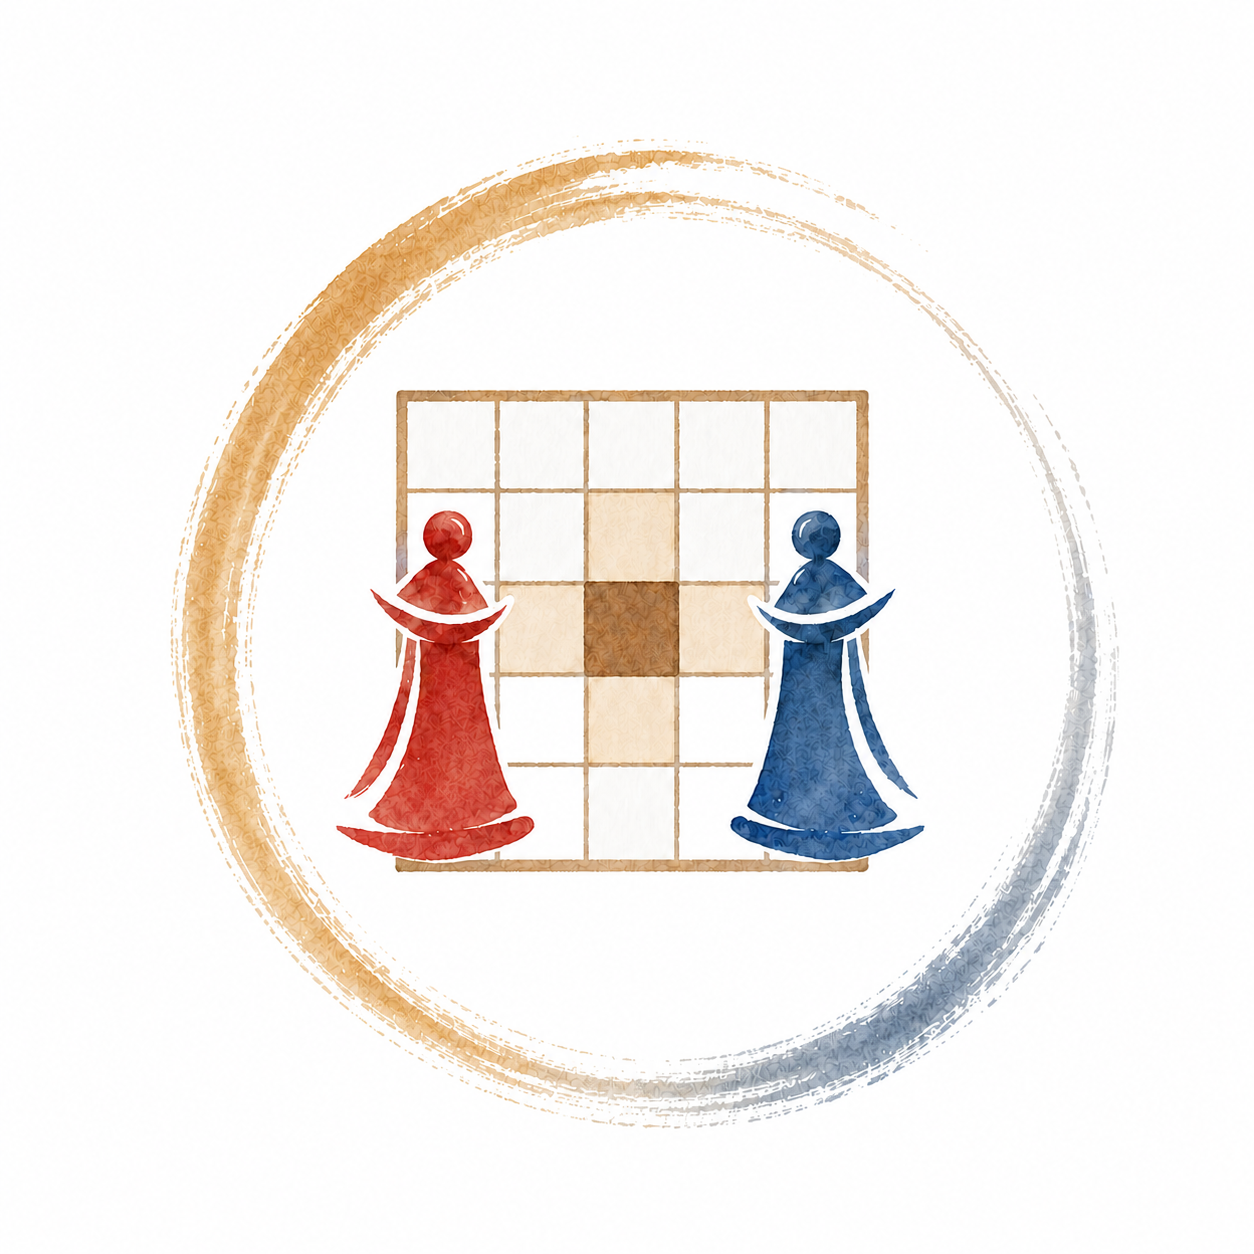
\includegraphics[width=0.6\textwidth]{imagenes/logo.png} 
 \vspace{0.5cm}

% título y subtítulo
{\Huge\bfseries \myTitle\\
}
\noindent\rule[-1ex]{\textwidth}{3pt}\\[3.5ex]
{\large\bfseries \mySubTitle\\[4cm]}
\end{minipage}


\vspace{2.5cm}
\noindent\hspace*{\centeroffset}\begin{minipage}{\textwidth}
\centering

\textbf{Autor}\\ {\myName}\\[2.5ex]
\textbf{Director}\\ {\myProf}\\[2cm]

\end{minipage}

\vspace{\stretch{2}}

 
\end{titlepage}





% -----------------------------------------------------------------------------
% Resumen en español
% -----------------------------------------------------------------------------

\cleardoublepage
\thispagestyle{empty}

\begin{center}
{\large\bfseries \myTitle: \mySubTitle}\\
\end{center}

\begin{center}
\myName\\
\end{center}

\noindent{\textbf{Palabras clave}: Onitama, agente inteligente, visión por computador, búsqueda adversarial, minimax, poda alfa-beta, detección de objetos, clasificación de imágenes.}\\

\vspace{0.7cm}
\noindent{\textbf{Resumen}}\\

Los juegos de tablero digitales suelen partir de un estado interno conocido por el programa. En una partida física, en cambio, el sistema debe reconstruir dicho estado a partir de la observación visual de la escena real. En este contexto, el propósito de este proyecto es permitir que un jugador humano dispute una partida física de Onitama contra un agente inteligente, manteniendo la manipulación real del tablero, las piezas y las cartas, y sincronizándola con una representación lógica fiable.

El sistema implementado integra un motor de reglas, un agente de inteligencia artificial, un módulo de visión por computador, una capa de sincronización físico-lógica y una interfaz gráfica de escritorio. El motor representa la partida y valida sus reglas; el agente selecciona jugadas mediante búsqueda adversarial basada en minimax con poda alfa-beta; y el módulo de visión detecta las piezas, clasifica las cartas visibles y reconstruye una observación estructurada de la escena. Dicha observación se estabiliza y se contrasta con las transiciones legales antes de aceptarse como nuevo estado confirmado.

La evaluación realizada analiza el comportamiento del agente, las optimizaciones de búsqueda, los modelos de visión y el funcionamiento integrado del sistema. Los resultados obtenidos confirman la consistencia del sistema completo, al mantener alineadas la evolución observada sobre el tablero real y la evolución interna utilizada para validar la partida y tomar decisiones.


% -----------------------------------------------------------------------------
% Resumen en inglés
% -----------------------------------------------------------------------------

\cleardoublepage
\thispagestyle{empty}

\begin{center}
{\large\bfseries Development of an intelligent system for Onitama with computer vision: Automatic reconstruction of the physical game state and move selection using Minimax with alpha-beta pruning}\\
\end{center}

\begin{center}
\myName\\
\end{center}

\noindent{\textbf{Keywords}: Onitama, intelligent agent, computer vision, adversarial search, minimax, alpha-beta pruning, object detection, image classification.}\\

\vspace{0.7cm}
\noindent{\textbf{Abstract}}\\

Digital board games usually start from an internal state known by the program. In a physical game, however, the system must reconstruct that state from the visual observation of the real scene. In this context, the purpose of this project is to allow a human player to play a physical game of Onitama against an intelligent agent, while preserving the real manipulation of the board, pieces, and cards, and synchronizing it with a reliable logical representation.

The implemented system integrates a rules engine, an artificial intelligence agent, a computer vision module, a physical-logical synchronization layer, and a desktop graphical interface. The engine represents the game and validates its rules; the agent selects moves using adversarial search based on minimax with alpha-beta pruning; and the vision module detects the pieces, classifies the visible cards, and reconstructs a structured observation of the scene. This observation is stabilized and compared against the legal transitions before being accepted as the new confirmed state.

The evaluation analyzes the behavior of the agent, the search optimizations, the vision models, and the integrated operation of the system. The results obtained confirm the consistency of the complete system, keeping the evolution observed on the real board aligned with the internal evolution used to validate the game and make decisions.


% -----------------------------------------------------------------------------
% Autorización para consulta en biblioteca
% -----------------------------------------------------------------------------

\chapter*{}
\thispagestyle{empty}

\noindent\rule[-1ex]{\textwidth}{2pt}\\[4.5ex]

Yo, \textbf{\myName}, alumno de la titulación INGENIERÍA INFORMÁTICA de la \textbf{Escuela Técnica Superior
de Ingenierías Informática y de Telecomunicación de la Universidad de Granada}, autorizo la
ubicación de la siguiente copia de mi Trabajo Fin de Grado en la biblioteca del centro para que pueda ser
consultada por las personas que lo deseen.

\vspace{6cm}

\noindent Fdo: \myName

\vspace{2cm}

\begin{flushright}
Granada, a 22 de junio de 2026.
\end{flushright}


% -----------------------------------------------------------------------------
% Informe y autorización del director
% -----------------------------------------------------------------------------

\chapter*{}
\thispagestyle{empty}

\noindent\rule[-1ex]{\textwidth}{2pt}\\[4.5ex]

D. \textbf{\myProf}, Profesor del Área de Ingeniería Informática del Departamento de Ciencias de la Computación e Inteligencia Artificial de la Universidad de Granada.

\vspace{0.5cm}

\textbf{Informa:}

\vspace{0.5cm}

Que el presente trabajo, titulado \textit{\textbf{\myTitle: \mySubTitle}},
ha sido realizado bajo su supervisión por \textbf{\myName}, y autoriza la defensa de dicho trabajo ante el tribunal
que corresponda.

\vspace{0.5cm}

Y para que conste, expide y firma el presente informe en Granada, a 22 de junio de 2026.

\vspace{1cm}

\textbf{El director:}

\vspace{5cm}

\noindent \textbf{\myProf}


% -----------------------------------------------------------------------------
% Agradecimientos
% -----------------------------------------------------------------------------

\chapter*{Agradecimientos}
\thispagestyle{empty}

\vspace{1cm}

En primer lugar, quiero agradecer a mi tutor, Salvador García López, por su orientación, disponibilidad y seguimiento durante el desarrollo de este Trabajo Fin de Grado. Su gran profesionalidad y experiencia han sido esenciales para idear y estructurar el proyecto. Me ha aportado visión y consejos muy valiosos en cada una de las etapas del proceso.

También quiero dar las gracias a mi familia, por su apoyo constante a lo largo de estos años. Mis padres y mi hermano son pilares fundamentales en mi vida, que me han aportado siempre la confianza, el ánimo y la tranquilidad necesarios para seguir avanzando. Son fuente de gran inspiración y todo un ejemplo a seguir. Gracias de corazón.

No me puedo olvidar de mis amigos y compañeros, que me han acompañado durante toda mi etapa universitaria, e incluso algunos desde mucho antes. Mi paso por la ETSIIT ha sido mucho más fácil a su lado. Gracias por la ayuda compartida, el apoyo y por sacarme una sonrisa siempre que nos juntamos.

Finalmente, me gustaría agradecer a todas las personas que han formado parte de esta etapa tan bonita de mi vida y me han visto crecer tanto académica como personalmente. Es una suerte haber tenido el privilegio de llegar hasta aquí.

\frontmatter
\tableofcontents
\listoffigures
\listoftables
\mainmatter
\setlength{\parskip}{5pt}

\chapter{Introducción}
\label{chap:introduccion}

%==============================================================================
% 1.1. Contexto y motivación
% =============================================================================
\section{Contexto y motivación}
\label{sec:contexto-motivacion}

Los juegos de tablero han ocupado un lugar destacado en el desarrollo de la inteligencia artificial. Sus reglas precisas y la necesidad de tomar decisiones frente a un adversario permiten estudiar el comportamiento de sistemas capaces de analizar posiciones, anticipar posibles respuestas y seleccionar acciones.

El interés por construir programas capaces de jugar se remonta a los orígenes de la inteligencia artificial. En 1950, Claude Shannon planteó algunos de los principios fundamentales para programar un ordenador que jugara al ajedrez \cite{shannon1950chess}. Décadas más tarde, en 1997, el sistema Deep Blue desarrollado por IBM derrotó al entonces campeón mundial Garri Kaspárov \cite{ibm_deep_blue}. Otro hito especialmente relevante se produjo con AlphaGo, que combinó técnicas de aprendizaje profundo y búsqueda para abordar el juego del Go y logró superar a jugadores profesionales de máximo nivel \cite{silver2016alphago}. Este último caso tuvo una gran repercusión pública y mostró de forma clara cómo un sistema de inteligencia artificial podía abordar con éxito un juego de estrategia especialmente complejo.

En la mayoría de las implementaciones informáticas de juegos de tablero, la partida se desarrolla sobre una representación completamente digital, de modo que el programa conoce directamente su estado. Sin embargo, la visión por computador permite conectar estas capacidades con juegos desarrollados sobre tableros reales. Un ejemplo de esta línea de trabajo es el sistema propuesto por Wölflein y Arandjelović para reconstruir posiciones de ajedrez a partir de fotografías, transformando la disposición física de las piezas en una representación utilizable por un motor de juego \cite{wolflein2021chessState}.

Este planteamiento permite incorporar herramientas automáticas de análisis sin sustituir el soporte material del juego ni exigir que el jugador reproduzca manualmente cada movimiento en una interfaz digital. El ordenador puede participar en la partida mientras el usuario continúa manipulando las piezas y cartas reales, conservando así la interacción física que caracteriza a los juegos de mesa. La posibilidad de relacionar una partida observada mediante una cámara con una representación digital constituye una de las principales motivaciones del presente trabajo.

La elección de Onitama responde tanto a su interés estratégico como a la viabilidad de desarrollar un sistema completo con medios técnicos asumibles dentro del proyecto. Frente a juegos tradicionalmente utilizados en inteligencia artificial, como el ajedrez o el Go, Onitama constituye un caso de estudio menos habitual. Su tablero de \(5 \times 5\) casillas, el número reducido de piezas y el uso de un conjunto limitado de cartas visibles permiten representar la partida, procesar visualmente sus componentes y ejecutar búsquedas y partidas automáticas en un ordenador portátil convencional.

Esta escala manejable no implica que la toma de decisiones resulte trivial. La carta utilizada en cada turno pasa posteriormente al oponente, por lo que una acción modifica tanto la posición del tablero como las opciones futuras de ambos jugadores. Además, la existencia de dos condiciones de victoria introduce objetivos complementarios. Onitama ofrece así un equilibrio adecuado entre originalidad, profundidad estratégica y viabilidad técnica.


%==============================================================================
% 1.2. Planteamiento del problema
% =============================================================================
\section{Planteamiento del problema}
\label{sec:planteamiento-problema}

En una implementación digital de un juego de tablero, el sistema dispone directamente de toda la información necesaria para gestionar la partida. La posición de las piezas, las cartas disponibles, el jugador activo y las acciones realizadas se encuentran representadas internamente, por lo que cada movimiento puede registrarse y validarse de forma inmediata. En una partida física, en cambio, esta información no está disponible de manera directa: el sistema solo puede acceder a ella a través de la observación de la escena real.

Esta diferencia introduce el problema central del proyecto. La imagen capturada por una cámara no equivale por sí misma al estado lógico de la partida. Una observación visual puede contener errores, elementos parcialmente ocultos o situaciones intermedias producidas mientras el jugador todavía está moviendo una pieza o intercambiando una carta. Por tanto, el sistema no puede aceptar cualquier configuración detectada como una posición válida, sino que debe interpretarla y contrastarla con las reglas del juego.

El problema no consiste únicamente en reconocer piezas o cartas de forma aislada. Para que la partida pueda desarrollarse correctamente, es necesario mantener sincronizadas dos representaciones de una misma realidad: la partida física, manipulada por el jugador sobre el tablero, y la partida lógica, utilizada por el programa para aplicar las reglas y tomar decisiones. La dificultad aparece precisamente en la relación entre ambas, ya que cada cambio observado debe corresponderse con una evolución legal desde el último estado confirmado.

Esta sincronización afecta tanto al turno del jugador humano como al turno de la inteligencia artificial. En el primer caso, el sistema debe comprobar que el movimiento realizado físicamente por el jugador es legal. En el segundo, el agente calcula una acción sobre la representación interna de la partida, pero dicha acción debe ejecutarse después sobre el tablero real y ser confirmada mediante la cámara. De este modo, la inteligencia artificial no actúa sobre una partida puramente digital, sino sobre una partida física que debe mantenerse coherente con su modelo interno.

El problema abordado en este trabajo puede resumirse, por tanto, como el desarrollo de un sistema capaz de conectar una partida física de Onitama con una representación digital fiable. Para ello, es necesario interpretar visualmente el tablero y las cartas, y validar los cambios observados de acuerdo con las reglas del juego. Sobre esta base, el sistema permite que un agente automático participe en la partida sin sustituir la interacción física del jugador con los componentes reales.


%==============================================================================
% 1.3. Objetivos del proyecto
% =============================================================================
\section{Objetivos del proyecto}
\label{sec:objetivos-proyecto}

El objetivo general de este trabajo es diseñar, implementar y evaluar un sistema inteligente que permita disputar una partida física de Onitama entre un jugador humano y un agente de inteligencia artificial.

Para alcanzar este objetivo general, se establecen los siguientes objetivos específicos:

\begin{itemize}
    \item Representar digitalmente el estado completo de una partida de Onitama, incluyendo la disposición de las piezas, el turno actual, las cartas disponibles para cada jugador y la carta lateral.

    \item Implementar un motor de reglas capaz de generar acciones legales, aplicar movimientos, resolver capturas, actualizar el intercambio de cartas y detectar las condiciones de victoria.

    \item Desarrollar un agente de inteligencia artificial capaz de seleccionar movimientos de forma automática a partir del estado actual de la partida y ofrecer distintos niveles de dificultad.

    \item Reconstruir el estado observado del tablero físico mediante técnicas de visión por computador, identificando tanto la posición, el color y el tipo de las piezas como las cartas visibles.

    \item Validar los cambios detectados en la escena física, comprobando que corresponden a transiciones legales desde el último estado confirmado de la partida.

    \item Coordinar el turno del jugador humano, la selección de la acción de la inteligencia artificial y la confirmación de su posterior ejecución sobre el tablero físico.

    \item Proporcionar una interfaz gráfica que permita configurar la partida, realizar las calibraciones necesarias, mostrar su evolución y guiar la interacción entre el usuario y el agente automático.

    \item Evaluar experimentalmente el comportamiento del agente de inteligencia artificial, el rendimiento de los modelos de visión y el funcionamiento conjunto de la aplicación.
\end{itemize}


%==============================================================================
% 1.4. Estructura de la memoria
% =============================================================================
\section{Estructura de la memoria}
\label{sec:estructura-memoria}

La memoria se organiza en siete capítulos, cuyo contenido se resume a continuación.

\begingroup
\titlespacing*{\paragraph}
    {0pt}
    {0.5\baselineskip}
    {1em}

\paragraph{Capítulo 1. Introducción.} Presenta el contexto y la motivación del trabajo, plantea el problema abordado y define los objetivos generales y específicos del proyecto. También describe la organización seguida en el resto de la memoria.

\paragraph{Capítulo 2. Fundamentos teóricos y tecnológicos.} Expone los conceptos necesarios para comprender el desarrollo del sistema. Incluye la representación digital de juegos de tablero, los fundamentos de la inteligencia artificial aplicada a juegos de dos jugadores, los algoritmos de búsqueda adversarial y las principales técnicas de visión por computador utilizadas para interpretar una escena física.

\paragraph{Capítulo 3. Fundamentos del juego Onitama.} Describe los componentes del juego, su configuración inicial, el desarrollo de los turnos y las condiciones de victoria. Además, analiza las implicaciones de estas reglas sobre la representación de la partida, la generación de movimientos y la observación de las piezas y cartas.

\paragraph{Capítulo 4. Análisis y diseño del sistema.} Recoge los requisitos funcionales y no funcionales, las restricciones de diseño y los principales casos de uso. También presenta la arquitectura general, los flujos de funcionamiento que coordinan los distintos componentes y la metodología seguida durante el desarrollo.

\paragraph{Capítulo 5. Implementación del sistema.} Detalla la organización del proyecto, incluyendo el enlace al código fuente desarrollado, y la construcción de sus principales componentes: el motor de juego, el agente de inteligencia artificial, el módulo de visión por computador, la lógica de sincronización, el control de ejecución, la interfaz gráfica y las herramientas auxiliares.

\paragraph{Capítulo 6. Experimentación y resultados.} Describe el entorno experimental y evalúa los componentes desarrollados. Se analizan las funciones heurísticas, las optimizaciones de búsqueda y los perfiles de dificultad del agente, así como el entrenamiento y el comportamiento de los modelos de visión y el funcionamiento conjunto del sistema.

\paragraph{Capítulo 7. Conclusiones y trabajo futuro.} Recoge las principales conclusiones obtenidas, valora el grado de cumplimiento de los objetivos, identifica las limitaciones del sistema y plantea posibles líneas de mejora y ampliación.

\endgroup

\chapter{Fundamentos teóricos y tecnológicos}
\label{chap:fundamentos-teoricos-tecnologicos}

Este capítulo presenta los conceptos teóricos y tecnológicos necesarios para contextualizar el desarrollo del proyecto. En primer lugar, se introduce la representación digital de juegos de tablero, prestando atención a cómo una partida física puede modelarse mediante estados, acciones y transiciones. A continuación, se revisan los fundamentos de la inteligencia artificial aplicada a juegos de dos jugadores, incluyendo los algoritmos de búsqueda adversarial más relevantes. Finalmente, se describen los conceptos principales de visión por computador necesarios para comprender la digitalización de un tablero físico mediante imágenes.

%==============================================================================
% 2.1. Juegos de tablero y representación digital
% =============================================================================
\section{Juegos de tablero y representación digital}
\label{sec:juegos-tablero-representacion-digital}

Los juegos de tablero constituyen un tipo concreto de juego de mesa en el que la partida se desarrolla sobre un espacio físico organizado, normalmente representado por un tablero dividido en posiciones, casillas o regiones. En torno a este espacio, los jugadores interactúan con piezas, fichas, cartas u otros componentes materiales siguiendo un conjunto de reglas que determina qué acciones son válidas, cómo se modifica la configuración de la partida y en qué condiciones esta llega a su fin.

Para que un juego de tablero pueda ser tratado por un sistema informático, es necesario abstraer sus elementos físicos en una representación digital. Esta representación no busca reproducir todos los detalles materiales del juego, como la apariencia exacta del tablero o la forma de sus componentes, sino conservar la información necesaria para aplicar sus reglas. De este modo, el tablero físico se convierte en una estructura formal sobre la que el programa puede comprobar movimientos, actualizar la partida y mantener una descripción coherente de su evolución.

Desde el punto de vista computacional, un juego puede definirse formalmente como un problema de búsqueda. Russell y Norvig describen esta formulación mediante una serie de componentes básicos~\cite{russell2020aima}:

\begin{itemize}
    \item \textbf{Estado inicial}: describe la configuración de partida e identifica el jugador al que corresponde mover.
    \item \textbf{Función sucesora}: devuelve, para un estado dado, las parejas formadas por un movimiento legal y el estado resultante tras aplicarlo.
    \item \textbf{Prueba terminal}: determina si la partida ha finalizado. Los estados en los que el juego ha terminado se denominan estados terminales.
    \item \textbf{Función de utilidad}: asigna un valor a los estados terminales, representando el resultado de la partida desde el punto de vista considerado.
\end{itemize}

A partir de esta formulación, una partida puede entenderse como una secuencia de estados conectados por acciones legales. Cada acción aplicada sobre un estado produce un nuevo estado, dando lugar a una transición. La partida avanza mediante estas transiciones hasta alcanzar, en su caso, un estado terminal asociado a un resultado.

El estado de juego representa una descripción lógica de una posición concreta de la partida. En un juego de tablero, este estado suele incluir la ubicación de las piezas, el turno actual, los recursos disponibles para cada jugador y cualquier otra información necesaria para aplicar correctamente las reglas.

A partir del estado actual, las reglas del juego determinan el conjunto de acciones legales. Esta distinción es fundamental, ya que no toda modificación posible del tablero constituye un movimiento válido. Aunque en un entorno físico un jugador pueda desplazar una pieza manualmente a una posición cualquiera, el modelo digital debe ser capaz de comprobar si esa acción respeta las restricciones del juego. En este sentido, la representación digital convierte las reglas en condiciones verificables por el sistema.

En los juegos por turnos, esta forma de modelar la evolución de la partida resulta especialmente natural. Cada jugador actúa en un momento determinado y cada movimiento modifica la posición sobre la que se tomará la siguiente decisión.

Además de representar posiciones intermedias, el modelo digital debe identificar cuándo la partida ha terminado. Para ello se reconocen estados terminales, es decir, situaciones en las que ya no es necesario continuar aplicando acciones. Estos estados suelen estar asociados a un resultado, como la victoria de un jugador, la derrota del otro o, en determinados juegos, un empate. La detección de estas condiciones permite validar el desarrollo de la partida y comunicar su desenlace al resto del sistema.

En conjunto, la representación digital proporciona una base formal sobre la que el sistema puede aplicar las reglas del juego y coordinar los módulos posteriores. Al separar la información relevante de los elementos físicos, el tablero deja de tratarse como un objeto material y pasa a describirse como una estructura lógica sobre la que pueden operar técnicas de inteligencia artificial y visión por computador.


%==============================================================================
% 2.2. Inteligencia artificial en juegos de dos jugadores
% =============================================================================
\section{Inteligencia artificial en juegos de dos jugadores}
\label{sec:inteligencia-artificial-juegos-dos-jugadores}

Una vez que un juego ha sido representado digitalmente mediante estados, acciones legales y transiciones, es posible aplicar técnicas de inteligencia artificial para seleccionar acciones de forma automática. En este contexto, el objetivo no consiste únicamente en ejecutar movimientos válidos, sino en escoger aquellos que resulten más favorables de acuerdo con el estado actual de la partida y sus posibles consecuencias futuras.

\subsection{Juegos como entornos adversariales}

Un juego de dos jugadores puede entenderse como un entorno de decisión en el que varios agentes actúan sobre un mismo estado compartido. Cada jugador elige sus acciones de acuerdo con sus propios objetivos, y dichas acciones modifican la situación sobre la que deberá decidir el rival en su turno. Por ello, el efecto de una jugada no puede analizarse de forma aislada, ya que también depende de las respuestas que puede provocar en el oponente.

En los juegos competitivos, esta interacción adquiere carácter adversarial, puesto que el avance de un jugador suele producirse en oposición al del otro. Una acción aparentemente favorable puede dejar una posición vulnerable si facilita una respuesta ventajosa del rival. En consecuencia, la decisión automática no debe limitarse a comprobar qué movimientos son legalmente posibles, sino que debe considerar la presencia de un oponente que también intenta mejorar su propia situación.

Esta perspectiva permite formular la partida como una secuencia de decisiones alternas entre dos participantes con intereses enfrentados. A partir de esta idea, resulta necesario estudiar qué propiedades del juego permiten modelar formalmente el problema y aplicar métodos de razonamiento adecuados para la toma de decisiones.


\subsection{Propiedades del modelo de juego}

Muchos juegos de tablero competitivos pueden estudiarse dentro de una categoría especialmente adecuada para la inteligencia artificial clásica: los juegos deterministas, por turnos, de información perfecta y, en muchos casos, de suma cero. Este marco permite describir la toma de decisiones de manera precisa y facilita el análisis de la partida desde un punto de vista computacional.

\begin{itemize}
    \item \textbf{Determinismo}: un juego es determinista cuando el resultado de una acción queda completamente determinado por el estado actual y por las reglas del juego. En este tipo de juegos no intervienen elementos aleatorios que alteren el resultado de una jugada, como dados, cartas ocultas robadas al azar o eventos externos. Por tanto, si se conoce el estado actual y la acción realizada, el estado resultante puede calcularse de forma precisa.

    \item \textbf{Turnos}: un juego por turnos es aquel en el que los jugadores actúan de forma alterna o secuencial. Cada jugador realiza una acción en su turno y modifica el estado sobre el que actuará el siguiente participante. Esta estructura se adapta de forma natural al razonamiento computacional, ya que la partida puede analizarse como una sucesión ordenada de decisiones.

    \item \textbf{Información perfecta}: en un juego de información perfecta, los jugadores conocen el estado completo de la partida en el momento de tomar una decisión. En este tipo de juegos, los agentes actúan secuencialmente y observan el estado del mundo antes de decidir qué acción realizar~\cite{poole2023foundations}. Esta propiedad los diferencia de juegos con información oculta o privada, donde un jugador puede desconocer parte de la situación real.

    \item \textbf{Suma cero}: en los juegos de suma cero, los intereses de los jugadores están directamente enfrentados. Una mejora en el resultado de un jugador implica un empeoramiento equivalente en el resultado del otro. En juegos de dos agentes de suma cero, una recompensa positiva para un agente se corresponde con una recompensa negativa para el otro~\cite{poole2023foundations}. Esta propiedad permite interpretar la partida como un conflicto directo entre objetivos opuestos.
\end{itemize}

Estas propiedades son especialmente relevantes en nuestro proyecto, ya que la partida puede describirse como una sucesión de turnos sin azar y con información visible para ambos jugadores. Esto permite que el sistema trate cada posición como un estado bien definido sobre el que aplicar reglas y seleccionar acciones legales.


%==============================================================================
% 2.3. Algoritmos de búsqueda adversarial
% =============================================================================
\section{Algoritmos de búsqueda adversarial}
\label{sec:algoritmos-busqueda-adversarial}

\subsection{Árbol de juego}

El árbol de juego es una representación de las posibles continuaciones de una partida a partir de un estado determinado. La raíz del árbol corresponde al estado actual, cada rama representa una acción legal y cada nodo hijo representa el estado resultante tras aplicar dicha acción. Al expandir sucesivamente los estados alcanzables, el árbol describe las diferentes secuencias de movimientos que podrían producirse durante la partida.

En un juego por turnos de dos jugadores, los niveles del árbol suelen alternar entre ambos participantes. Un nivel representa las decisiones disponibles para el jugador que debe mover en ese momento, mientras que el siguiente nivel representa las posibles respuestas del oponente. De este modo, el árbol no solo muestra las acciones inmediatas, sino también las consecuencias que pueden derivarse de ellas tras varios turnos.

Las hojas del árbol pueden corresponder a estados terminales, cuando la partida ha finalizado, o a estados intermedios cuando la búsqueda se detiene antes de llegar al final. En el primer caso, el valor del estado puede obtenerse directamente a partir del resultado de la partida. En el segundo caso, es necesario estimar la calidad de la posición mediante una función de evaluación, aspecto que se tratará más adelante.

Aunque el árbol de juego proporciona una representación clara del problema, su tamaño puede crecer rápidamente. Si en cada estado existen varias acciones legales, el número de nodos aumenta de forma exponencial con la profundidad de búsqueda. Esta expansión combinatoria hace que, en muchos juegos, no sea viable explorar todas las partidas posibles hasta llegar a estados terminales. Por este motivo, los algoritmos de búsqueda adversarial incorporan técnicas para seleccionar, limitar u optimizar la exploración del árbol~\cite{russell2020aima,poole2023foundations}.


\subsection{Algoritmo minimax}

El algoritmo minimax es uno de los métodos clásicos para la toma de decisiones en juegos de dos jugadores, deterministas, por turnos y de suma cero. El concepto minimax tiene su origen en la teoría de juegos, especialmente en los trabajos de John von Neumann sobre juegos de dos personas con intereses opuestos~\cite{kjeldsen2001minimax}. En inteligencia artificial, se utiliza habitualmente como un procedimiento de búsqueda sobre árboles de juego para seleccionar movimientos bajo la hipótesis de que ambos jugadores actúan de forma racional~\cite{russell2020aima,poole2023foundations}. En este contexto, un jugador intenta maximizar el valor de la posición, mientras que el adversario intenta minimizarlo.

El funcionamiento general del algoritmo puede resumirse en los siguientes pasos:

\begin{enumerate}
    \item Se construye, de forma explícita o implícita, el árbol de juego a partir del estado actual.
    \item Se asigna un valor a los nodos hoja, ya sea porque representan estados terminales o porque se ha alcanzado una profundidad máxima de búsqueda.
    \item En los niveles correspondientes al jugador maximizador, se selecciona el mayor valor entre los nodos sucesores.
    \item En los niveles correspondientes al jugador minimizador, se selecciona el menor valor entre los nodos sucesores.
    \item Los valores se propagan desde las hojas hacia la raíz, permitiendo elegir la acción inicial con mejor valor minimax.
\end{enumerate}

La Figura~\ref{fig:minimax-tree} muestra un ejemplo sencillo de propagación de valores. Los nodos hoja contienen evaluaciones numéricas de distintas posiciones. En primer lugar, cada nodo de minimización selecciona el menor valor entre sus hijos. Después, la raíz, correspondiente al jugador maximizador, selecciona el mayor valor entre los valores propagados por sus sucesores.

\vspace{0.5cm}

\begin{figure}[htbp]
\centering
\begin{tikzpicture}[
    level distance=1.4cm,
    level 1/.style={sibling distance=4.2cm},
    level 2/.style={sibling distance=1.8cm},
    every node/.style={
        draw,
        rounded corners,
        align=center,
        minimum width=1.2cm,
        minimum height=0.7cm
    },
    edge from parent/.style={draw, -latex}
]
\node {MAX\\$3$}
    child {node {MIN\\$3$}
        child {node {\hspace{1.5mm}$3$}}
        child {node {\hspace{1.5mm}$5$}}
    }
    child {node {MIN\\$2$}
        child {node {\hspace{1.5mm}$2$}}
        child {node {\hspace{1.5mm}$9$}}
    };
\end{tikzpicture}
\caption{Ejemplo de propagación de valores en el algoritmo minimax.}
\label{fig:minimax-tree}
\end{figure}
\vspace{1cm}


El Algoritmo~\ref{alg:minimax} muestra una versión simplificada de minimax, adaptada a una búsqueda con profundidad limitada a partir de la formulación clásica del algoritmo~\cite{russell2020aima}. La función recibe un estado, una profundidad restante y un indicador que determina si el turno corresponde al jugador maximizador o al minimizador. Si el estado es terminal o se ha alcanzado la profundidad límite, se devuelve una evaluación del estado. En caso contrario, se exploran las acciones legales y se propaga el valor máximo o mínimo según el jugador que deba actuar.

\vspace{0.3cm}
\begin{algorithm}[H]
\caption{Algoritmo minimax}
\label{alg:minimax}
\begin{algorithmic}[1]
\State \textbf{Entrada:} estado de juego $s$, profundidad restante $d$, indicador $maximizando$
\State \textbf{Salida:} valor estimado del estado $s$
\If{$s$ es terminal \textbf{o} $d = 0$}
    \State \Return $evaluar(s)$
\EndIf
\If{$maximizando$}
    \State $mejor \gets -\infty$
    \ForAll{acción legal $a$ en $s$}
        \State $s' \gets resultado(s, a)$
        \State $mejor \gets \max(mejor, minimax(s', d - 1, false))$
    \EndFor
    \State \Return $mejor$
\Else
    \State $mejor \gets +\infty$
    \ForAll{acción legal $a$ en $s$}
        \State $s' \gets resultado(s, a)$
        \State $mejor \gets \min(mejor, minimax(s', d - 1, true))$
    \EndFor
    \State \Return $mejor$
\EndIf
\end{algorithmic}
\end{algorithm}

En juegos de suma cero, minimax puede expresarse también mediante la formulación \textbf{negamax}. Esta variante aprovecha que el valor de una posición para un jugador es el opuesto del valor de esa misma posición para el adversario. De este modo, en lugar de alternar explícitamente entre una función de maximización y otra de minimización, la búsqueda puede formularse como una única función que maximiza el valor negativo del estado resultante desde la perspectiva del rival. Conceptualmente, negamax no cambia el criterio de decisión de minimax, sino que ofrece una forma más compacta de expresarlo en juegos con utilidad opuesta para ambos jugadores.

La principal ventaja de minimax es que proporciona un criterio claro para decidir en juegos adversariales. Sin embargo, su coste computacional puede ser elevado, ya que el número de nodos crece rápidamente con la profundidad de búsqueda. Por ello, en la práctica suele combinarse con límites de profundidad, funciones heurísticas y técnicas de optimización.


\subsection{Poda alfa-beta}

La poda alfa-beta es una optimización del algoritmo minimax que permite reducir el número de nodos explorados en el árbol de juego sin modificar la decisión final obtenida. La idea principal consiste en dejar de analizar aquellas ramas que no pueden influir en el valor que finalmente será seleccionado por minimax. Por tanto, alfa-beta no cambia el criterio de decisión del algoritmo, sino la eficiencia con la que se recorre el árbol~\cite{russell2020aima,poole2023foundations}.

El algoritmo mantiene dos valores durante la búsqueda: $\alpha$ y $\beta$. El valor $\alpha$ representa la mejor alternativa encontrada hasta el momento para el jugador maximizador, mientras que $\beta$ representa la mejor alternativa encontrada hasta el momento para el jugador minimizador. Si durante la exploración se detecta que un nodo no puede mejorar la decisión ya disponible para alguno de los jugadores, el resto de sus sucesores puede descartarse sin necesidad de evaluarlos.

El funcionamiento de la poda alfa-beta puede resumirse en los siguientes pasos:

\begin{enumerate}
    \item Se recorre el árbol de juego de forma similar a minimax, alternando entre niveles de maximización y minimización.
    \item Durante la búsqueda, se actualiza $\alpha$ con el mejor valor encontrado hasta el momento para el jugador maximizador.
    \item Del mismo modo, se actualiza $\beta$ con el mejor valor encontrado hasta el momento para el jugador minimizador.
    \item Si en algún momento se cumple que $\alpha \geq \beta$, la rama actual deja de poder afectar al resultado final y se interrumpe su exploración.
    \item El valor devuelto por el algoritmo es el mismo que devolvería minimax, pero normalmente habiendo evaluado menos nodos.
\end{enumerate}

La Figura~\ref{fig:alphabeta-pruning} muestra un ejemplo simplificado de esta idea. Una vez que el primer subárbol ha proporcionado a la raíz una alternativa con valor $3$, el segundo nodo de minimización encuentra un sucesor con valor $2$. Dado que el jugador minimizador escogería como máximo un valor menor o igual que $2$ en ese subárbol, dicha rama ya no puede mejorar la opción disponible para el jugador maximizador. Por ello, el resto de sucesores del nodo puede descartarse sin alterar la decisión final.

\vspace{0.5cm}
\begin{figure}[H]
\centering
\begin{tikzpicture}[
    level distance=1.5cm,
    level 1/.style={sibling distance=5.0cm},
    level 2/.style={sibling distance=2.0cm},
    normal/.style={
        draw,
        rounded corners,
        align=center,
        minimum width=1.3cm,
        minimum height=0.75cm,
    },
    pruned/.style={
        draw=red!70,
        rounded corners,
        align=center,
        minimum width=1.3cm,
        minimum height=0.75cm,
        fill=red!10,
        text=red!70
    },
    edge from parent/.style={draw, -latex},
    prunededge/.style={draw=red!70, dashed, -latex}
]

\node[normal] {MAX\\$3$}
    child {node[normal] {MIN\\$3$}
        child {node[normal] {\hspace{1.5mm}$3$}}
        child {node[normal] {\hspace{1.5mm}$5$}}
    }
    child {node[normal] {MIN\\$2$}
        child {node[normal] {\hspace{1.5mm}$2$}}
        child[prunededge] {node[pruned] {\hspace{1.5mm}podado}}
    };

\end{tikzpicture}
\caption{Ejemplo de poda alfa-beta en un árbol minimax.}
\label{fig:alphabeta-pruning}
\end{figure}
\vspace{0.8cm}

El Algoritmo~\ref{alg:alphabeta} muestra una versión simplificada de minimax con poda alfa-beta. Al igual que en el caso anterior, se utiliza una profundidad máxima de búsqueda y una función de evaluación para los estados terminales o para aquellos estados en los que se alcanza el límite de profundidad. La diferencia principal respecto a minimax es la actualización de los valores $\alpha$ y $\beta$, que permiten detectar cuándo una rama puede ser descartada.

\begin{algorithm}[H]
\caption{Minimax con poda alfa-beta}
\label{alg:alphabeta}
\begin{algorithmic}[1]
\State \textbf{Entrada:} estado de juego $s$, profundidad restante $d$, valores \textcolor{blue}{$\alpha$ y $\beta$}, indicador $maximizando$
\State \textbf{Salida:} valor estimado del estado $s$
\If{$s$ es terminal \textbf{o} $d = 0$}
    \State \Return $evaluar(s)$
\EndIf
\If{$maximizando$}
    \State $mejor \gets -\infty$
    \ForAll{acción legal $a$ en $s$}
        \State $s' \gets resultado(s, a)$
        \State $mejor \gets \max(mejor, alphabeta(s', d - 1, \textcolor{blue}{\alpha}, \textcolor{blue}{\beta}, false))$
        \State \textcolor{blue}{$\alpha \gets \max(\alpha, mejor)$}
        \If{\textcolor{blue}{$\alpha \geq \beta$}}
            \State \textcolor{blue}{\textbf{break}}
        \EndIf
    \EndFor
    \State \Return $mejor$
\Else
    \State $mejor \gets +\infty$
    \ForAll{acción legal $a$ en $s$}
        \State $s' \gets resultado(s, a)$
        \State $mejor \gets \min(mejor, alphabeta(s', d - 1, \textcolor{blue}{\alpha}, \textcolor{blue}{\beta}, true))$
        \State \textcolor{blue}{$\beta \gets \min(\beta, mejor)$}
        \If{\textcolor{blue}{$\alpha \geq \beta$}}
            \State \textcolor{blue}{\textbf{break}}
        \EndIf
    \EndFor
    \State \Return $mejor$
\EndIf
\end{algorithmic}
\end{algorithm}

La poda alfa-beta constituye una de las optimizaciones clásicas de minimax en árboles de juego~\cite{knuth1975alphabeta}. Su utilidad práctica no depende únicamente de las condiciones de corte descritas, sino también de su integración con estrategias que mejoran el recorrido del árbol. Estas técnicas, presentadas más adelante, no modifican el criterio de decisión del algoritmo, pero pueden reducir el coste computacional de la búsqueda y permitir alcanzar mayores profundidades en motores de juego.


\subsection{Profundidad limitada y funciones heurísticas}

Aunque minimax y la poda alfa-beta proporcionan un marco claro para tomar decisiones en juegos adversariales, en muchos juegos no resulta viable explorar el árbol completo hasta alcanzar estados terminales. El número de nodos crece rápidamente con la profundidad de búsqueda, ya que cada acción legal puede dar lugar a nuevos estados y cada uno de ellos genera, a su vez, nuevas posibilidades. Por este motivo, incluso en juegos con reglas relativamente sencillas, analizar todas las partidas posibles puede ser computacionalmente inasumible.

Para abordar esta limitación, es habitual utilizar una búsqueda con profundidad limitada. En lugar de expandir el árbol hasta el final de la partida, el algoritmo se detiene tras alcanzar una profundidad máxima. En este contexto, dicha profundidad suele medirse en \emph{ply}, término que representa un movimiento individual de uno de los jugadores dentro del árbol de juego. Por tanto, una búsqueda de varios \emph{ply} permite analizar secuencias alternas de acciones propias y respuestas del adversario. Esta limitación reduce el coste computacional y permite controlar el tiempo dedicado a la toma de decisiones.

El uso de profundidad limitada plantea un nuevo problema: al detener la búsqueda antes de alcanzar estados terminales, el algoritmo ya no dispone de un resultado definitivo de victoria, derrota o empate. Por tanto, es necesario estimar la calidad de las posiciones alcanzadas en la frontera de búsqueda. Esta estimación se realiza mediante una función heurística de evaluación, que asigna un valor numérico a un estado no terminal en función de características consideradas relevantes para el juego~\cite{russell2020aima,poole2023foundations}.

Una función heurística no garantiza conocer el resultado real de la partida desde una posición concreta, sino que proporciona una aproximación útil para orientar la búsqueda. En juegos de tablero, estas funciones suelen combinar distintos criterios, entre los que pueden encontrarse:

\begin{itemize}
    \item \textbf{Ventaja material}: diferencia entre las piezas o recursos disponibles para cada jugador.
    \item \textbf{Movilidad}: número o calidad de las acciones legales disponibles.
    \item \textbf{Seguridad}: grado de protección de piezas o posiciones importantes.
    \item \textbf{Control del tablero}: influencia sobre zonas relevantes del espacio de juego.
    \item \textbf{Proximidad a la victoria}: cercanía a una condición que permita finalizar favorablemente la partida.
\end{itemize}

La elección de estos factores depende de las características del juego y condiciona en gran medida el comportamiento del agente.

Desde el punto de vista de minimax, la función heurística sustituye a la función de utilidad cuando la búsqueda no llega a un estado terminal. Los valores estimados en la frontera del árbol se propagan entonces hacia la raíz mediante el mismo procedimiento de maximización y minimización. De este modo, el algoritmo puede seleccionar una acción aunque solo haya explorado una parte limitada del espacio de juego.

La calidad de una inteligencia artificial basada en búsqueda depende, por tanto, de un equilibrio entre profundidad y evaluación. Una búsqueda más profunda permite considerar consecuencias más lejanas, pero requiere más tiempo de cómputo. Una función heurística más precisa puede compensar parcialmente una búsqueda menos profunda, aunque también puede introducir errores si valora incorrectamente una posición. Este equilibrio entre coste computacional y calidad de la evaluación es uno de los aspectos fundamentales en el diseño de agentes para juegos de tablero.


\subsection{Técnicas de optimización de la búsqueda}

Además de la poda alfa-beta, los motores basados en búsqueda suelen incorporar técnicas complementarias para mejorar la eficiencia del recorrido del árbol o la calidad de las evaluaciones realizadas en la frontera de búsqueda. Schaeffer agrupa muchas de estas mejoras en torno a tres ideas principales: ordenar mejor los movimientos, reducir el tamaño de la ventana de búsqueda y reutilizar información obtenida en búsquedas anteriores~\cite{schaeffer1989historyHeuristic}. Estas técnicas no modifican el problema de decisión adversarial, pero permiten aprovechar mejor el tiempo de cómputo disponible.

\begin{itemize}
    \item \textbf{Ordenación de movimientos}: la eficacia de alfa-beta depende en gran medida del orden en que se exploran las acciones. Si las jugadas más prometedoras se analizan primero, los cortes pueden producirse antes y se reduce el número de nodos evaluados. Por ello, muchos motores utilizan heurísticas para priorizar ciertos movimientos, como capturas, amenazas o jugadas que en búsquedas anteriores han producido buenos resultados. Schaeffer estudia precisamente la \emph{history heuristic}, una técnica que acumula información sobre movimientos que han sido útiles en otras partes del árbol y la utiliza para ordenar movimientos en nodos posteriores~\cite{schaeffer1989historyHeuristic}.

    \item \textbf{Tablas de transposición}: en un árbol de juego, una misma posición puede alcanzarse mediante distintas secuencias de movimientos. Las tablas de transposición aprovechan esta propiedad almacenando información de estados ya explorados, como el valor calculado, la profundidad de búsqueda utilizada o el mejor movimiento encontrado. Si la misma posición aparece de nuevo, el algoritmo puede reutilizar esa información para evitar búsquedas repetidas, ajustar los límites de alfa-beta o probar primero un movimiento previamente considerado prometedor~\cite{schaeffer1989historyHeuristic, marsland1986gameTreePruning}.

    \item \textbf{Profundización iterativa}: en lugar de ejecutar directamente una búsqueda a una profundidad fija, la profundización iterativa realiza búsquedas sucesivas de profundidad creciente. Por ejemplo, primero se explora a un ply, después a dos, luego a tres, y así sucesivamente hasta alcanzar el límite deseado o agotar el tiempo disponible. Aunque pueda parecer redundante, esta técnica permite disponer siempre de una mejor jugada parcial si la búsqueda debe detenerse y, además, proporciona información útil para ordenar movimientos en iteraciones posteriores~\cite{schaeffer1989historyHeuristic, marsland1986gameTreePruning}.

    \item \textbf{Ventanas de aspiración}: en una búsqueda alfa-beta habitual, los valores iniciales de $\alpha$ y $\beta$ pueden cubrir un intervalo muy amplio. Las ventanas de aspiración utilizan una ventana más estrecha alrededor de una estimación previa del valor esperado de la posición. Si el valor real cae dentro de esa ventana, la búsqueda puede completarse con menor coste; si queda fuera, es necesario repetir la búsqueda con límites más amplios. Esta técnica puede mejorar la eficiencia, aunque depende de que la estimación inicial sea suficientemente precisa~\cite{schaeffer1989historyHeuristic, marsland1986gameTreePruning}.

    \item \textbf{Búsqueda quiescente}: al utilizar profundidad limitada, el algoritmo puede detenerse en una posición tácticamente inestable, por ejemplo justo antes de una captura o de una amenaza importante. Evaluar directamente ese estado puede producir una estimación engañosa. La búsqueda quiescente intenta reducir este problema extendiendo selectivamente la búsqueda en posiciones no estables hasta alcanzar estados más tranquilos, donde la función de evaluación pueda aplicarse con mayor fiabilidad. Marsland relaciona esta técnica con la reducción del efecto horizonte, que aparece cuando una pérdida inevitable queda artificialmente desplazada más allá de la profundidad máxima de búsqueda~\cite{marsland1986gameTreePruning}.
\end{itemize}

En conjunto, los algoritmos y técnicas descritos en esta sección proporcionan la base del agente de inteligencia artificial desarrollado en este proyecto. Al modelar Onitama como un juego adversarial de turnos alternos, cada posición puede analizarse mediante un árbol de posibles continuaciones. Sin embargo, para que esta búsqueda sea viable en la práctica, es necesario combinar el criterio de decisión de minimax con una profundidad limitada, una función heurística de evaluación, poda alfa-beta y técnicas de optimización del recorrido. De este modo, el sistema puede seleccionar acciones legales de forma automática, equilibrando la calidad de la decisión con el tiempo de cálculo disponible.


%==============================================================================
% 2.4. Captura y normalización de la escena física.
% =============================================================================
\section{Captura y normalización de la escena física}
\label{sec:captura-normalizacion-escena-fisica}


\subsection{Captura visual del tablero}

La aplicación de visión por computador a un tablero físico parte de una diferencia fundamental entre la escena real y la información disponible para el sistema: la cámara no recibe directamente objetos, casillas o posiciones, sino una imagen bidimensional. Esta imagen es el resultado de un proceso de formación en el que intervienen la geometría de la escena, la iluminación, las propiedades de las superficies, la óptica de la cámara y la discretización realizada por el sensor~\cite{szeliski2022computerVision}. Por ello, el análisis visual del tablero debe partir de una observación condicionada por el modo en que la escena física se proyecta y se registra como imagen.

En un entorno físico, la observación del tablero no suele ser completamente limpia ni constante. Pequeños cambios en la posición de la cámara, variaciones de luz, sombras, reflejos sobre las cartas o movimientos de la mano del jugador pueden modificar de forma significativa la imagen capturada, aunque la situación lógica del juego no haya cambiado. Esta diferencia entre la estabilidad del juego y la variabilidad de la imagen es uno de los principales retos al utilizar una cámara como mecanismo de entrada.

Los juegos de tablero presentan, no obstante, una ventaja importante desde el punto de vista visual: la escena suele organizarse alrededor de una superficie plana y de regiones espaciales bien definidas. La existencia de un tablero permite buscar una referencia geométrica estable sobre la que interpretar el resto de elementos. En lugar de analizar la imagen como una escena completamente libre, puede aprovecharse la estructura del tablero para restringir el problema a una zona concreta y relacionar los elementos observados con regiones conocidas de la superficie de juego.

Existen trabajos que plantean la reconstrucción o el seguimiento del estado de juegos de tablero físicos a partir de imágenes, especialmente en el caso del ajedrez~\cite{wolflein2021chessState,koray2016chessTracking,masouris2023endToEndChess}. Estos enfoques ilustran una estrategia habitual en tableros físicos: localizar primero la superficie de juego, transformarla después a una cuadrícula regular y utilizar esa organización espacial como base para el análisis posterior de sus elementos. Aunque las características visuales de cada juego sean distintas, este planteamiento muestra la importancia de separar la normalización geométrica de la interpretación visual.

En consecuencia, antes de abordar la identificación de los componentes del juego, conviene reducir la ambigüedad introducida por la forma en que la escena física aparece en la imagen. Para ello, el análisis puede apoyarse en la propia geometría del tablero, utilizando su estructura regular como referencia para obtener una vista más controlada de la superficie de juego.


\subsection{Corrección geométrica de la imagen}

Cuando el tablero se observa desde una posición oblicua, su forma rectangular y la distribución uniforme de sus regiones no se conservan directamente en la imagen capturada. Un tablero rectangular puede aparecer como un cuadrilátero deformado por la perspectiva, de modo que las casillas no tienen por qué ocupar áreas iguales y las distancias aparentes entre regiones pueden variar.

Si la superficie del tablero se aproxima como un plano, esta deformación puede tratarse mediante una transformación proyectiva u homografía~\cite{szeliski2022computerVision}. Esta transformación permite relacionar la imagen capturada por la cámara con una vista normalizada del tablero, en la que sus regiones quedan organizadas dentro de un sistema de coordenadas más regular.

\vspace{0.5cm}
\begin{figure}[H]
    \centering
    \begin{tikzpicture}[scale=0.9, every node/.style={font=\small}]

        % Left: perspective-distorted board
        \coordinate (A) at (0,0.15);
        \coordinate (B) at (3.6,0.65);
        \coordinate (C) at (2.75,2.65);
        \coordinate (D) at (-0.45,1.75);

        \draw[thick] (A) -- (B) -- (C) -- (D) -- cycle;

        % Internal vertical-like grid lines
        \foreach \t in {0.2,0.4,0.6,0.8} {
            \draw[gray] ($(A)!\t!(B)$) -- ($(D)!\t!(C)$);
        }

        % Internal horizontal-like grid lines
        \foreach \t in {0.2,0.4,0.6,0.8} {
            \draw[gray] ($(A)!\t!(D)$) -- ($(B)!\t!(C)$);
        }

        \node at (1.45,-0.55) {Imagen capturada};

        % Arrow
        \draw[-{Latex}, thick] (4.25,1.3) -- (5.95,1.3);
        \node at (5.1,1.68) {homografía};

        % Right: normalized board
        \draw[thick] (6.6,0) rectangle (9.0,2.4);

        \foreach \x in {7.08,7.56,8.04,8.52} {
            \draw[gray] (\x,0) -- (\x,2.4);
        }

        \foreach \y in {0.48,0.96,1.44,1.92} {
            \draw[gray] (6.6,\y) -- (9.0,\y);
        }

        \node at (7.8,-0.55) {Vista normalizada};

    \end{tikzpicture}
    \caption{Normalización geométrica de un tablero aplicando homografía.}
\end{figure}

Una homografía establece una correspondencia entre puntos de dos vistas de una misma superficie plana. Esta relación puede expresarse como:

\[
\tilde{\mathbf{x}}' \sim \mathbf{H}\tilde{\mathbf{x}}
\]

donde:

\begin{itemize}
    \item \(\tilde{\mathbf{x}}\) representa un punto de la imagen original en coordenadas homogéneas;
    \item \(\tilde{\mathbf{x}}'\) representa el punto correspondiente en la vista normalizada;
    \item \(\mathbf{H}\) es una matriz \(3 \times 3\) que define la homografía;
    \item el símbolo \(\sim\) indica igualdad hasta un factor de escala.
\end{itemize}

Szeliski describe este tipo de transformación como una transformación proyectiva bidimensional que conserva la rectitud de las líneas, propiedad especialmente útil cuando se trabaja con superficies planas y estructuras regulares como tableros~\cite{szeliski2022computerVision}.

Para calcular esta transformación es necesario disponer de correspondencias entre puntos de la imagen capturada y puntos conocidos de la vista de destino. En un tablero físico, estas correspondencias pueden proceder de referencias espaciales estables, como esquinas, marcas o puntos característicos de la superficie. Una vez estimada la homografía, la imagen puede transformarse hacia una vista normalizada, en la que las regiones del tablero quedan organizadas de forma más uniforme.

Esta normalización no resuelve por sí sola la identificación de los componentes del juego, pero reduce la variabilidad espacial introducida por la perspectiva. En el contexto de este proyecto, permite aproximar la observación del tablero físico a una representación más regular, donde las regiones de imagen pueden relacionarse con posiciones concretas del tablero y servir de base para las técnicas de detección y clasificación descritas en la siguiente sección.


%==============================================================================
% 2.5. Reconocimiento visual mediante clasificación y detección.
% =============================================================================
\section{Reconocimiento visual mediante clasificación y detección}
\label{sec:reconocimiento-visual-clasificacion-deteccion}


\subsection{Modelos aprendidos para el análisis de imágenes}

El reconocimiento visual basado en modelos aprendidos parte de la idea de sustituir reglas manuales por modelos entrenados con ejemplos. En lugar de describir explícitamente todas las formas, colores o patrones que caracterizan a un elemento visual, el modelo ajusta su comportamiento a partir de imágenes representativas del problema. Este planteamiento resulta especialmente útil en problemas con alta variabilidad visual, donde resulta difícil anticipar manualmente todas las apariencias posibles de un mismo objeto.

Esta variabilidad es habitual en imágenes capturadas en entornos reales. Un mismo elemento puede aparecer con cambios de iluminación, perspectiva, escala, orientación, fondo u oclusión parcial. Además, objetos pertenecientes a una misma clase no siempre presentan una apariencia idéntica, mientras que elementos de clases distintas pueden compartir rasgos visuales parecidos. Por ello, los modelos aprendidos permiten abordar el análisis de imágenes desde una perspectiva más flexible que la definición manual de reglas fijas.

El entrenamiento de estos modelos puede plantearse de distintas formas. En muchas tareas de reconocimiento visual se utiliza aprendizaje supervisado, especialmente cuando se dispone de ejemplos asociados a una respuesta esperada, como la clase de una imagen o la localización de un objeto dentro de ella. En este caso, el modelo produce una predicción para cada entrada, la compara con la respuesta correcta y ajusta sus parámetros para reducir el error. Una vez entrenado, puede aplicar lo aprendido a imágenes nuevas, siempre que estas mantengan una relación suficiente con los ejemplos empleados durante el entrenamiento.

Dentro de este enfoque, el aprendizaje profundo ha adquirido una gran importancia en visión por computador. Estos modelos, basados en redes neuronales con múltiples capas, aprenden representaciones internas a partir de los ejemplos de entrenamiento, reduciendo la dependencia de descriptores visuales definidos manualmente. En lugar de especificar explícitamente qué rasgos deben buscarse en la imagen, el propio modelo ajusta sus parámetros para extraer patrones útiles para la tarea visual considerada~\cite{lecun2015deepLearning}.

Sobre esta base se desarrollan tareas de reconocimiento visual como la clasificación de imágenes y la detección de objetos, que se describen a continuación.


\subsection{Clasificación de imágenes}

La clasificación de imágenes es una tarea de reconocimiento visual en la que se asigna una etiqueta a una imagen completa o a una región previamente delimitada. El modelo analiza el contenido visual de la entrada y estima qué categoría se corresponde mejor con él. Por ello, resulta especialmente adecuada cuando el elemento de interés ya ha sido separado antes de aplicar el modelo, como ocurre en problemas basados en recortes o regiones de interés.


De forma general, un clasificador recibe una imagen como entrada y produce una puntuación para cada una de las clases posibles. La predicción final se obtiene seleccionando la clase con mayor confianza. Este planteamiento permite convertir una observación visual en una etiqueta discreta, siempre que el contenido relevante esté suficientemente representado en la imagen de entrada.

Una forma habitual de construir este tipo de clasificadores es mediante redes neuronales convolucionales. Estas redes aplican filtros sobre regiones locales de la imagen y reutilizan dichos filtros en distintas posiciones, lo que permite reconocer rasgos visuales similares aunque aparezcan en zonas diferentes de la entrada. Esta arquitectura resulta especialmente adecuada para imágenes porque aprovecha su estructura espacial mediante conexiones locales, pesos compartidos y capas sucesivas~\cite{lecun2015deepLearning}. 

La Figura~\ref{fig:clasificacion-imagenes-cnn} resume de forma esquemática este flujo de clasificación.

\vspace{0.5cm}
\begin{figure}[H]
    \centering
    \resizebox{0.96\textwidth}{!}{
    \begin{tikzpicture}[
        every node/.style={font=\small},
        arrow/.style={-{Latex}, thick, draw=black!80},
        label/.style={font=\small, align=center, text width=2.8cm, anchor=north}
    ]

        \def\LabelY{-0.62}

        % -------------------------------------------------
        % 1. Imagen o recorte
        % -------------------------------------------------
        \fill[gray!5, rounded corners] (0,0) rectangle (2.4,2.4);
        \draw[black, rounded corners, thick] (0,0) rectangle (2.4,2.4);
        \foreach \x in {0.48,0.96,1.44,1.92} {
            \draw[gray] (\x,0) -- (\x,2.4);
        }
        \foreach \y in {0.48,0.96,1.44,1.92} {
            \draw[gray] (0,\y) -- (2.4,\y);
        }
        \node[label] at (1.2,\LabelY) {Imagen o recorte};

        % Flecha 1
        \draw[arrow] (2.4,1.2) -- (3.8,1.2);

        % -------------------------------------------------
        % 2. Red convolucional
        % -------------------------------------------------
        \draw[rounded corners, fill=gray!35, draw=black, thick] (4.20,0.30) rectangle (5.75,1.85);
        \draw[rounded corners, fill=gray!25, draw=black, thick] (4.40,0.45) rectangle (5.95,2.00);
        \draw[rounded corners, fill=gray!10, draw=black, thick] (4.60,0.60) rectangle (6.15,2.15);

        \node[label] at (5.18,\LabelY) {Red neuronal convolucional};

        % Flecha 2
        \draw[arrow] (6.15,1.2) -- (7.55,1.2);

        % -------------------------------------------------
        % 3. Puntuaciones por clase
        % -------------------------------------------------
        \fill[gray!5, rounded corners] (7.55,0.40) rectangle (9.45,2.00);
        \draw[black, rounded corners, thick] (7.55,0.40) rectangle (9.45,2.00);

        % Barras centradas dentro del recuadro
        \draw[fill=gray!35, draw=black!70, thick] (7.82,0.65) rectangle (8.08,1.55);
        \draw[fill=gray!25, draw=black!70, thick] (8.22,0.65) rectangle (8.48,1.05);
        \draw[fill=gray!50, draw=black!80, thick] (8.62,0.65) rectangle (8.88,1.80);
        \draw[fill=gray!25, draw=black!70, thick] (9.02,0.65) rectangle (9.28,0.92);

        \node[label] at (8.50,\LabelY) {Puntuaciones por clase};

        % Flecha 3
        \draw[arrow] (9.45,1.2) -- (10.85,1.2);

        % -------------------------------------------------
        % 4. Predicción final
        % -------------------------------------------------
        \fill[gray!10, rounded corners] (10.85,0.75) rectangle (12.65,1.65);
        \draw[black, rounded corners, thick] (10.85,0.75) rectangle (12.65,1.65);
        \node[font=\small\bfseries, text=black!85] at (11.75,1.2) {Clase};

        \node[label] at (11.75,\LabelY) {Predicción final};

    \end{tikzpicture}
    }
    \caption{Esquema general de clasificación de imágenes mediante una red neuronal convolucional.}
    \label{fig:clasificacion-imagenes-cnn}
\end{figure}

La principal ventaja de la clasificación es su simplicidad conceptual: el sistema recibe una imagen ya delimitada y devuelve una identidad visual. Esta aproximación resulta adecuada cuando la región de interés está bien definida, pero no cubre por sí sola los casos en los que el sistema debe analizar una escena completa con varios elementos relevantes. En esos casos, además de reconocer la categoría de cada objeto, es necesario estimar su posición en la imagen, lo que conduce a la tarea de detección de objetos.

\subsection{Detección de objetos}

La detección de objetos amplía el planteamiento anterior al incorporar esta información espacial al reconocimiento visual. En esta tarea, el modelo no trabaja únicamente con una imagen o recorte ya delimitado, sino con una escena que puede contener varios objetos. Por ello, la salida de un detector suele expresarse como un conjunto de predicciones, donde cada una incluye una caja delimitadora, una etiqueta de clase y un valor de confianza asociado~\cite{szeliski2022computerVision}.

Esta salida permite transformar la imagen en una descripción estructurada de la escena. Cada caja delimitadora aproxima la posición y el tamaño de un objeto, mientras que la clase asociada indica su identidad visual y el valor de confianza refleja la seguridad de la predicción.

Entre los detectores modernos destaca YOLO, acrónimo de \textit{You Only Look Once}. Se trata de una familia de detectores basada en redes neuronales convolucionales, diseñada para procesar la imagen completa en una sola pasada y de manera eficiente. Su idea principal consiste en tratar la detección como un problema unificado: el modelo predice directamente múltiples cajas delimitadoras junto con sus niveles de confianza y sus probabilidades de clase. Después, las predicciones menos fiables o redundantes se descartan para conservar únicamente las detecciones finales más plausibles~\cite{redmon2016yolo}. 

La Figura~\ref{fig:deteccion-objetos} ilustra el tipo de salida que produce un detector de este tipo.

\vspace{0.5cm}
\begin{figure}[H]
    \centering
    \resizebox{0.80\textwidth}{!}{
    \begin{tikzpicture}[
        every node/.style={font=\small}
    ]

        % Imagen de fondo
        \fill[gray!10] (0,0) rectangle (11,6);
        \draw[rounded corners, thick] (0,0) rectangle (11,6);

        % Objetos en la escena
        % Objeto 1
        \fill[red!35] (2.0,1.7) circle (0.55);

        % Objeto 2
        \fill[blue!35] (6.8,3.9) -- (7.5,2.8) -- (6.1,2.8) -- cycle;

        % Objeto 3
        \fill[green!60!black] (8.3,1.3) rectangle (9.2,2.2);

        % Cajas delimitadoras
        \draw[red, very thick] (1.2,0.9) rectangle (2.9,2.6);
        \draw[blue, very thick] (5.8,2.5) rectangle (7.8,4.5);
        \draw[green!50!black, very thick] (7.9,0.9) rectangle (9.6,2.6);

        % Etiquetas ajustadas automáticamente al texto
        \node[
            fill=red,
            rounded corners=1pt,
            inner sep=2pt,
            anchor=south west,
            text=white,
            font=\scriptsize\bfseries
        ] at (1.2,2.6) {Clase A \, (0.93)};

        \node[
            fill=blue,
            rounded corners=1pt,
            inner sep=2pt,
            anchor=south west,
            text=white,
            font=\scriptsize\bfseries
        ] at (5.8,4.5) {Clase B \, (0.89)};

        \node[
            fill=green!50!black,
            rounded corners=1pt,
            inner sep=2pt,
            anchor=south west,
            text=white,
            font=\scriptsize\bfseries
        ] at (7.9,2.6) {Clase C \, (0.95)};

    \end{tikzpicture}
    }
    \caption{Ejemplo esquemático de detección de objetos sobre una imagen, con cajas delimitadoras, clases y niveles de confianza.}
    \label{fig:deteccion-objetos}
\end{figure}

La dificultad principal de la detección es que combina una decisión semántica y una decisión geométrica. El modelo debe reconocer la categoría de cada objeto, pero también estimar una región que represente de forma razonable su ubicación en la imagen. Esta doble exigencia hace que la tarea sea sensible a objetos pequeños, oclusiones parciales, solapamientos o elementos muy próximos entre sí. Aun así, constituye una herramienta especialmente valiosa cuando se necesita recuperar tanto la identidad de los elementos visuales como su disposición espacial dentro de la escena.


\subsection{Reconstrucción del estado observado}

Las etapas anteriores permiten obtener predicciones visuales sobre la escena capturada, pero la detección y la clasificación no constituyen por sí mismas el objetivo final del sistema. Para que la información obtenida mediante la cámara resulte útil, es necesario transformarla en una representación estructurada de lo que se observa en la partida física.

La reconstrucción del estado observado consiste en combinar la localización de los elementos visibles con la identidad asignada por los modelos de reconocimiento. En un tablero físico, la normalización geométrica permite relacionar zonas de la imagen con regiones conocidas de la superficie de juego. Sobre esta base, el proceso puede entenderse como una secuencia de transformaciones: primero se obtienen predicciones visuales sobre los elementos presentes, después se relacionan con posiciones o regiones del tablero y, finalmente, se organizan en una descripción discreta de la observación.

En el caso de \textit{Onitama}, esta transformación debe recoger principalmente dos tipos de información visual:

\begin{itemize}
    \item \textbf{Piezas}: es necesario determinar qué regiones del tablero están ocupadas e identificar el color y el tipo de cada pieza, diferenciando entre maestros y estudiantes.
    \item \textbf{Cartas}: es necesario reconocer la identidad de las cartas visibles, ya que forman parte de la información observable que condiciona el desarrollo de la partida.
\end{itemize}

El resultado de este proceso no es simplemente una imagen anotada, sino una descripción discreta de la observación visual. Sin embargo, dicha descripción debe entenderse como una estimación obtenida a partir de la imagen capturada, no como el estado lógico definitivo de la partida. La observación puede verse afectada por errores de perspectiva, oclusiones parciales, reflejos, recortes imprecisos o predicciones incorrectas de los modelos.

Por ello, la información reconstruida desde la imagen puede requerir etapas posteriores de comprobación y estabilización antes de utilizarse como entrada fiable del sistema. De este modo, la reconstrucción del estado observado actúa como enlace entre el reconocimiento visual y los módulos internos del proyecto, traduciendo las salidas de detección y clasificación en datos estructurados que puedan ser tratados computacionalmente.


%==============================================================================
% ANTECEDENTES Y TRABAJOS RELACIONADOS  (OPCIONAL)
% =============================================================================
% Para esta última seccion quizas se puede meter algo así como ejemplos de 
% proyectos similares o aplicaciones concretas de visión por computador en juegos de tablero. 
% Como el AlphaGo.


\chapter{Fundamentos del juego Onitama}
\label{chap:fundamentos-juego-onitama}

%==============================================================================
% 3.1. Descripción general del juego
% =============================================================================
\section{Descripción general del juego}
\label{sec:descripcion-general-onitama}

\textit{Onitama} es un juego de mesa abstracto de estrategia para dos jugadores, diseñado por Shimpei Sato y publicado originalmente en Japón en 2014. En este trabajo se toma como referencia la edición y el reglamento de Arcane Wonders, una de las editoriales principales en su distribución internacional \cite{onitama_bgg,onitama_rulebook}.

La propuesta del juego se basa en un enfrentamiento directo entre dos escuelas de artes marciales. Cada jugador controla a un maestro y a sus discípulos sobre un tablero reducido, tratando de superar al rival mediante movimientos precisos y decisiones cuidadosamente planificadas. Esta premisa permite presentar el juego de forma sencilla, sin necesidad de una gran cantidad de piezas, reglas o excepciones.

El aspecto más característico de \textit{Onitama} es que los movimientos disponibles no dependen de cada pieza de forma individual, sino de un conjunto limitado de cartas visibles. Estas cartas cambian durante la partida, por lo que cada turno afecta tanto a la posición actual del tablero como a las opciones que estarán disponibles más adelante. Por ello, aunque el juego utiliza pocos elementos, cada decisión tiene consecuencias tácticas inmediatas y estratégicas a medio plazo.

Estas características hacen que \textit{Onitama} sea un caso adecuado para el sistema desarrollado en este trabajo, al combinar una estructura discreta, un funcionamiento por turnos y elementos físicos claramente observables. Por ello, en las siguientes secciones se describen los elementos que componen una partida, la configuración inicial, el desarrollo de los turnos, las condiciones de victoria y las implicaciones que estas reglas tienen sobre el sistema implementado.


%==============================================================================
% 3.2. Elementos y configuración inicial
% =============================================================================
\section{Elementos y configuración inicial}
\label{sec:elementos-configuracion-inicial}

\textit{Onitama} utiliza un conjunto reducido de componentes, lo que facilita la comprensión de la partida desde el primer momento. Los elementos principales son el tablero, las piezas de ambos jugadores y las cartas de movimiento.

\begin{itemize}
    \item \textbf{Tablero}: está formado por una cuadrícula de \(5 \times 5\) casillas. En la fila inicial de cada jugador existe una casilla especial, situada en el centro, denominada templo. Esta casilla interviene tanto en la colocación inicial del maestro como en una de las condiciones de victoria.

    \item \textbf{Piezas}: cada jugador dispone de cinco piezas de un mismo color: un maestro y cuatro estudiantes. Todas las piezas utilizan las mismas cartas de movimiento, por lo que el tipo de pieza no determina cómo se desplaza. No obstante, el maestro tiene una importancia especial dentro de los objetivos de la partida.

    \item \textbf{Cartas de movimiento}: el juego base incluye dieciséis cartas. Cada carta representa un patrón de desplazamientos posibles que puede aplicarse a cualquiera de las piezas del jugador activo. Estas cartas no pertenecen de forma permanente a un jugador, sino que rotan entre ambos durante la partida.
\end{itemize}

La configuración inicial se realiza a partir de estos elementos y determina la situación desde la que comienza la partida:

\begin{enumerate}
    \item Cada jugador coloca su maestro en la casilla de templo correspondiente.
    \item Los cuatro estudiantes se sitúan en las casillas restantes de esa misma fila, a los lados del maestro.
    \item Se barajan las dieciséis cartas de movimiento.
    \item Cada jugador recibe dos cartas visibles, que forman su mano inicial.
    \item Se revela una quinta carta, que se coloca en el lateral del tablero.
    \item El sello de color de esa quinta carta determina qué jugador realiza el primer turno.
    \item Las cartas restantes no se utilizan durante esa partida.
\end{enumerate}

La Figura~\ref{fig:configuracion-inicial-onitama} muestra de forma esquemática esta disposición inicial, incluyendo la posición de las piezas, las cartas visibles de cada jugador y la carta lateral.

\begin{figure}[htbp]
    \centering

    \begin{tikzpicture}[
        board/.style={
            line width=0.5pt
        },
        templeBlue/.style={
            fill=blue!15
        },
        templeRed/.style={
            fill=red!15
        },
        studentBlue/.style={
            circle,
            draw,
            fill=blue!30,
            minimum size=0.42cm,
            inner sep=0pt
        },
        studentRed/.style={
            circle,
            draw,
            fill=red!30,
            minimum size=0.42cm,
            inner sep=0pt
        },
        masterBlue/.style={
            circle,
            draw,
            fill=blue!40,
            minimum size=0.52cm,
            inner sep=0pt,
            font=\scriptsize\bfseries
        },
        masterRed/.style={
            circle,
            draw,
            fill=red!40,
            minimum size=0.52cm,
            inner sep=0pt,
            font=\scriptsize\bfseries
        },
        card/.style={
            rectangle,
            draw,
            rounded corners=2pt,
            fill=white,
            minimum width=1.20cm,
            minimum height=1.15cm,
            font=\scriptsize
        },
        labelText/.style={
            font=\scriptsize
        }
    ]

        \node[labelText] at (2.5,6.65) {Cartas del jugador azul};
        \node[card] at (1.8,5.75) {$C_3$};
        \node[card] at (3.2,5.75) {$C_4$};

        \node[labelText] at (6.55,3.15) {Carta lateral};
        \node[card] at (6.55,2.30) {$C_L$};

        \fill[templeRed] (2,0) rectangle (3,1);
        \fill[templeBlue] (2,4) rectangle (3,5);

        \draw[board] (0,0) rectangle (5,5);
        \foreach \i in {1,2,3,4} {
            \draw[board] (\i,0) -- (\i,5);
            \draw[board] (0,\i) -- (5,\i);
        }

        \foreach \x in {0.5,1.5,3.5,4.5} {
            \node[studentBlue] at (\x,4.5) {};
        }
        \node[masterBlue] at (2.5,4.5) {M};

        \foreach \x in {0.5,1.5,3.5,4.5} {
            \node[studentRed] at (\x,0.5) {};
        }
        \node[masterRed] at (2.5,0.5) {M};

        \node[card] at (1.8,-0.75) {$C_1$};
        \node[card] at (3.2,-0.75) {$C_2$};
        \node[labelText] at (2.5,-1.65) {Cartas del jugador rojo};

    \end{tikzpicture}

    \caption{Representación esquemática de la configuración inicial de una partida de \textit{Onitama}. Las casillas coloreadas de la columna central corresponden a los templos de cada jugador.}
    \label{fig:configuracion-inicial-onitama}
\end{figure}


%==============================================================================
% 3.3. Desarrollo de una partida
% =============================================================================
\section{Desarrollo de una partida}
\label{sec:desarrollo-partida-onitama}

Una vez establecida la configuración inicial, la partida avanza mediante turnos alternos. En cada turno, el jugador activo debe realizar dos pasos principales: primero mueve una de sus piezas utilizando una carta de movimiento y, después, intercambia la carta utilizada por la carta situada en el lateral del tablero \cite{onitama_rulebook}.

\subsubsection*{Movimiento y ataque}

El primer paso del turno consiste en elegir una de las dos cartas disponibles y aplicar uno de sus movimientos a una pieza propia. La pieza seleccionada puede ser tanto el maestro como cualquiera de los estudiantes, ya que en \textit{Onitama} los desplazamientos no dependen del tipo de pieza, sino de la carta utilizada.

Las cartas representan movimientos relativos respecto a la posición actual de la pieza. En cada carta, la casilla central indica la posición de origen y las casillas marcadas muestran los posibles destinos. Además, el patrón debe interpretarse desde la perspectiva del jugador que realiza el movimiento, por lo que una misma carta puede producir desplazamientos opuestos para cada jugador.

Para que un movimiento sea legal, deben cumplirse las siguientes condiciones:

\begin{itemize}
    \item La casilla de destino debe encontrarse dentro de los límites del tablero.
    \item La casilla de destino no puede estar ocupada por una pieza propia.
    \item El desplazamiento debe corresponderse con una de las posiciones indicadas por la carta seleccionada.
\end{itemize}

Si la casilla de destino está ocupada por una pieza rival, dicha pieza es capturada y se retira del tablero. Las piezas situadas entre la casilla de origen y la de destino no bloquean el movimiento, ya que el desplazamiento se considera directo. Del mismo modo, solo se captura una pieza rival cuando la pieza movida termina exactamente sobre su casilla.

\subsubsection*{Intercambio de cartas}

Después de resolver el movimiento, el jugador debe intercambiar la carta que acaba de utilizar. La carta usada se coloca en el lateral del tablero, orientada hacia el jugador contrario, y el jugador activo toma la carta que se encontraba previamente en esa posición. A partir de ese momento, dicha carta pasa a formar parte de sus opciones disponibles para turnos posteriores.

Este intercambio es una de las mecánicas más características de \textit{Onitama}. Cada turno no solo modifica la posición de las piezas, sino también el conjunto de cartas que estarán disponibles más adelante. Por tanto, una decisión puede ser favorable por el movimiento que permite en ese instante, pero también debe valorarse por la carta que entrega al rival.

Existe además un caso especial: si el jugador activo no puede realizar ningún movimiento legal con ninguna de sus dos cartas, debe pasar el turno. No obstante, incluso en esta situación debe escoger una de sus cartas e intercambiarla por la carta lateral, de manera que la circulación de cartas continúa aunque ninguna pieza se desplace \cite{onitama_rulebook}.


%==============================================================================
% 3.4. Condiciones de victoria
% =============================================================================
\section{Condiciones de victoria}
\label{sec:condiciones-victoria-onitama}

La partida finaliza cuando uno de los jugadores cumple una de las dos condiciones de victoria definidas por el reglamento. Ambas condiciones están relacionadas con el maestro, lo que diferencia a esta pieza del resto y le otorga un papel central dentro de la estrategia del juego \cite{onitama_rulebook}.

Las dos formas de ganar son las siguientes:

\begin{itemize}
    \item \textbf{Captura del maestro rival}: un jugador gana si una de sus piezas termina su movimiento sobre la casilla ocupada por el maestro del oponente. Esta condición es denominada en el reglamento como \textit{Way of the Stone}.
    
    \item \textbf{Llegada al templo contrario}: un jugador también gana si consigue mover su propio maestro hasta la casilla de templo del oponente. Esta condición es denominada en el reglamento como \textit{Way of the Stream}.
\end{itemize}

Estas dos vías de victoria generan objetivos complementarios. Por un lado, cada jugador debe proteger a su maestro para evitar una derrota inmediata por captura. Por otro lado, también puede buscar una victoria posicional avanzando con su maestro hasta el templo rival. Los estudiantes no activan directamente la victoria por templo, pero resultan importantes para controlar casillas, bloquear opciones del oponente y apoyar tanto la defensa como el avance del maestro.


%==============================================================================
% 3.5. Implicaciones para el sistema desarrollado
% =============================================================================
\section{Implicaciones para el sistema desarrollado}
\label{sec:implicaciones-sistema-onitama}

Las reglas descritas en las secciones anteriores condicionan directamente el diseño del sistema desarrollado. Al tratarse de un juego por turnos, con tablero discreto, piezas diferenciadas y cartas visibles, la aplicación debe coordinar varios módulos: motor de juego, inteligencia artificial, visión por computador e integración con la partida física.

Desde el punto de vista del motor de juego, una posición de \textit{Onitama} no queda definida únicamente por la colocación de las piezas sobre el tablero. También es necesario conocer qué jugador debe mover, qué cartas tiene disponibles cada jugador y qué carta se encuentra en el lateral. Por tanto, el estado de la partida debe integrar información espacial, información relativa a las piezas e información asociada a las cartas.

De forma resumida, el motor debe contemplar los siguientes aspectos:

\begin{itemize}
    \item La ocupación de cada una de las \(25\) casillas del tablero.
    \item El color y el tipo de cada pieza, diferenciando entre maestro y estudiantes.
    \item El jugador al que corresponde realizar el turno.
    \item Las dos cartas disponibles para cada jugador.
    \item La carta situada en el lateral.
    \item La generación de movimientos legales a partir de las cartas disponibles.
    \item La aplicación de capturas, intercambios de cartas y cambios de turno.
    \item La detección de las condiciones de victoria.
\end{itemize}

En el caso de la inteligencia artificial, estas reglas determinan el conjunto de acciones que puede analizar en cada turno. Las acciones legales generadas por el motor forman las alternativas de búsqueda, mientras que las condiciones de victoria permiten identificar estados terminales. Además, la importancia del maestro y la rotación de cartas influyen en la valoración estratégica de cada posición, ya que una jugada no solo debe evaluarse por el movimiento inmediato que produce, sino también por las cartas que deja disponibles para turnos posteriores.

Desde el punto de vista de la visión por computador, el sistema debe extraer del tablero físico la información necesaria para reconstruir una situación de partida válida. Esto implica identificar qué casillas están ocupadas, a qué jugador pertenece cada pieza, si se trata de un maestro o de un estudiante, y qué cartas se encuentran visibles en la disposición de la partida.

Por último, la integración entre visión, motor de reglas e inteligencia artificial exige comprobar que las observaciones obtenidas desde la cámara sean coherentes con la evolución legal del juego. No basta con detectar una configuración aislada del tablero, sino que es necesario verificar que el cambio observado respecto al estado anterior corresponde a una acción válida. Esta validación permite reducir errores derivados del ruido visual, de oclusiones temporales o de movimientos incompletos del jugador humano.

Estas implicaciones sirven como punto de partida para el análisis y diseño del sistema, que se aborda en el siguiente capítulo.


\chapter{Análisis y diseño del sistema}
\label{chap:analisis-diseno-sistema}



\chapter{Implementación del sistema}
\label{chap:implementacion-sistema}



\chapter{Experimentación y resultados}
\label{chap:experimentacion-resultados}



\chapter{Conclusiones y trabajo futuro}
\label{chap:conclusiones-trabajo-futuro}

%==============================================================================
% 7.1. Conclusiones
% =============================================================================
\section{Conclusiones}
\label{sec:conclusiones}

El desarrollo de este proyecto ha permitido construir un sistema completo para disputar una partida física de Onitama entre un jugador humano y un agente de inteligencia artificial. La solución obtenida no se limita a implementar las reglas del juego o a seleccionar movimientos de forma automática, sino que conecta estas capacidades con la observación de un tablero real mediante visión por computador y con una interfaz que coordina la interacción durante la partida.

La principal aportación del trabajo se encuentra en la integración entre la dimensión física y la representación lógica del juego. Una imagen capturada por la cámara no constituye por sí sola un estado válido, por lo que ha sido necesario distinguir entre la observación visual y el estado confirmado de la partida. La estabilización de las observaciones y su comparación con las transiciones permitidas por el motor de reglas permiten mantener la coherencia entre ambas representaciones y evitar que lecturas incompletas o incorrectas modifiquen indebidamente la partida.

Esta separación de responsabilidades también ha resultado fundamental para la organización del sistema. El motor de juego, el agente de inteligencia artificial, el módulo de visión, la lógica de sincronización, el control de ejecución y la interfaz gráfica se han desarrollado como componentes diferenciados, pero coordinados mediante representaciones y operaciones comunes. Este enfoque ha facilitado su validación independiente y ha permitido abordar de forma progresiva la integración final.

Onitama ha resultado un caso de estudio adecuado para este propósito. Su escala permite representar y analizar la partida con recursos computacionales accesibles, mientras que la rotación de las cartas y las distintas condiciones de victoria mantienen una complejidad estratégica suficiente para justificar el desarrollo de un agente de búsqueda. Del mismo modo, el reducido número de piezas y cartas visibles hace viable la reconstrucción del estado mediante una cámara, sin eliminar los retos propios de una escena física real.

En conjunto, el trabajo muestra que es posible incorporar un agente inteligente a un juego de tablero físico sin sustituir sus componentes materiales por una interfaz completamente digital. El sistema desarrollado actúa como enlace entre la percepción visual, la aplicación de las reglas y la toma automática de decisiones, manteniendo al jugador humano como responsable de la manipulación del tablero. El resultado constituye una base funcional sobre la que pueden realizarse nuevas mejoras tanto en la robustez visual como en la autonomía y capacidad de decisión del sistema.


%==============================================================================
% 7.2. Cumplimiento de los objetivos
% =============================================================================
\section{Cumplimiento de los objetivos}
\label{sec:cumplimiento-objetivos}

El objetivo general definido al inicio de la memoria consistía en diseñar, implementar y evaluar un sistema inteligente que permitiera disputar una partida física de Onitama entre un jugador humano y un agente de inteligencia artificial. Tras el desarrollo realizado, este objetivo puede considerarse cumplido, ya que se ha construido una aplicación capaz de representar la partida, observar el tablero físico, validar la evolución del juego y coordinar la actuación del agente automático.

El cumplimiento de este objetivo general se concreta en los distintos objetivos específicos planteados:

\begin{itemize}
    \item \textbf{Representación digital de la partida.} Se ha definido una representación completa del estado de Onitama, incluyendo el tablero, las piezas, el jugador activo, las cartas disponibles para cada jugador y la carta lateral. Esta representación ha servido como base común para el motor de reglas, la inteligencia artificial y la sincronización con la observación visual.

    \item \textbf{Implementación del motor de reglas.} Se ha desarrollado un motor capaz de generar acciones legales, aplicar movimientos, resolver capturas, actualizar el intercambio de cartas y detectar las dos condiciones de victoria del juego. Este componente actúa como referencia lógica del sistema y garantiza que la evolución interna de la partida respete las reglas de Onitama.

    \item \textbf{Desarrollo del agente de inteligencia artificial.} Se ha implementado un agente basado en búsqueda adversarial, con funciones heurísticas de evaluación y distintas técnicas de optimización. Además, se han definido perfiles de dificultad que permiten ajustar el comportamiento del agente en función de la profundidad de búsqueda empleada.

    \item \textbf{Reconstrucción visual del estado físico.} Se ha construido un módulo de visión por computador capaz de procesar imágenes capturadas por una cámara, detectar las piezas sobre el tablero y clasificar las cartas visibles. A partir de esta información, el sistema puede generar una observación estructurada de la escena física.

    \item \textbf{Validación de los cambios observados.} Se ha incorporado una capa de sincronización que no acepta directamente cualquier observación visual, sino que la estabiliza y la compara con las transiciones legales generadas por el motor. De este modo, el sistema puede distinguir entre estados válidos, observaciones sin cambio y configuraciones incoherentes con la evolución de la partida.

    \item \textbf{Coordinación de los turnos de juego.} Se ha desarrollado una lógica de sesión que coordina el turno del jugador humano, la selección de la jugada de la inteligencia artificial y la confirmación de su ejecución física sobre el tablero. Esta coordinación permite que el agente participe en una partida real sin que el juego se reduzca a una simulación puramente digital.

    \item \textbf{Desarrollo de la interfaz gráfica.} Se ha implementado una aplicación de escritorio que permite configurar la partida, realizar las calibraciones necesarias, visualizar el estado del juego, mostrar las cartas y guiar al usuario durante la interacción con el agente automático.

    \item \textbf{Evaluación experimental.} Se han realizado pruebas sobre los principales componentes del sistema. En particular, se ha evaluado el comportamiento del agente mediante torneos y benchmarks de búsqueda, se han entrenado y validado los modelos de visión por computador y se ha comprobado el funcionamiento conjunto de la aplicación en condiciones reales de uso.
\end{itemize}

En conjunto, los objetivos planteados se han alcanzado dentro del alcance definido para el proyecto. El sistema resultante permite jugar físicamente a Onitama con asistencia de inteligencia artificial y visión por computador, aunque su funcionamiento sigue condicionado por las restricciones propias del montaje físico, la cámara y los modelos visuales empleados.


%==============================================================================
% 7.3. Principales resultados
% =============================================================================
\section{Principales resultados}
\label{sec:principales-resultados}

La evaluación experimental permitió comparar las distintas alternativas desarrolladas y justificar la configuración final del sistema. Los resultados más relevantes se resumen a continuación.

\paragraph{Comparación de las funciones heurísticas.}
En el agente de inteligencia artificial, la función heurística \texttt{v3} obtuvo el mejor comportamiento en los cuatro torneos realizados. Su tasa de puntuación se situó alrededor del 65\,\% en profundidad 3 y entre el 72\,\% y el 76\,\% en profundidad 4, superando tanto a \texttt{v1} como a \texttt{v2} en los enfrentamientos directos. Estos resultados respaldan el uso de una evaluación dependiente de la fase de la partida, capaz de adaptar la importancia de los distintos criterios estratégicos conforme evoluciona el juego.

\paragraph{Impacto de las optimizaciones de búsqueda.}
El análisis realizado mostró que no todas las optimizaciones implementadas aportaban el mismo beneficio en el escenario estudiado. La ordenación de movimientos fue la técnica con un efecto más claro, ya que su desactivación incrementó progresivamente el tiempo y el número de nodos explorados al aumentar la profundidad. La tabla de transposición presentó un comportamiento menos estable, mientras que la profundización iterativa y las ventanas de aspiración añadieron coste en las búsquedas a profundidad fija utilizadas. La configuración final, que conserva la ordenación de movimientos y desactiva estas tres técnicas, redujo el tiempo total respecto a la configuración completa en un 18.4\,\%, un 19.4\,\% y un 31.2\,\% para las profundidades 3, 4 y 5, respectivamente.

\paragraph{Efecto de la búsqueda quiescente.}
La búsqueda quiescente produjo una mejora clara en la calidad del agente. En los torneos comparativos, la configuración sin esta extensión obtuvo una tasa de puntuación próxima al 33\,\%, mientras que la profundidad quiescente 2 alcanzó valores cercanos al 62\,\% en los dos bloques de semillas evaluados. El aumento del tiempo por decisión fue reducido dentro del contexto de una partida interactiva, por lo que esta configuración se mantuvo en los perfiles definitivos.

\paragraph{Perfiles de dificultad.}
Los torneos entre niveles confirmaron una separación coherente entre los perfiles definidos. El perfil fácil obtuvo una tasa de puntuación del 12.38\,\%, el perfil medio alcanzó el 49.88\,\% y el perfil difícil llegó al 87.75\,\%. Los tiempos medios por decisión permanecieron por debajo de una décima de segundo incluso en el nivel difícil. La combinación de la heurística \texttt{v3}, una profundidad principal de 5 y una profundidad quiescente de 2 permitió así alcanzar un nivel de juego elevado sin perjudicar la fluidez de la partida. En las partidas manuales realizadas durante el desarrollo, este perfil ofreció además un reto considerable frente a jugadores familiarizados con Onitama.

% Los apartados sobre los modelos de visión y la valoración conjunta
% se completarán cuando finalicen las pruebas en condiciones reales
% y la validación funcional del sistema integrado.
Faltan los dos últimos apartados!!

%==============================================================================
% 7.4. Limitaciones
% =============================================================================
\section{Limitaciones}
\label{sec:limitaciones}

Aunque el sistema desarrollado cumple los objetivos planteados, su funcionamiento está condicionado por varios factores que deben tenerse en cuenta al interpretar los resultados y valorar su posible uso en otros entornos.

\paragraph{Condiciones de captura y generalización visual.}
El rendimiento del módulo de visión depende de factores como la iluminación, el enfoque, los reflejos, las oclusiones y la visibilidad de las piezas y cartas. Además, los modelos se han entrenado con los componentes físicos y las condiciones de captura empleadas durante el desarrollo. Por ello, cambios significativos en el tablero, las piezas, las cartas o el entorno podrían reducir la fiabilidad y requerir nuevos datos de entrenamiento o ajustes adicionales.

\paragraph{Calibración y montaje físico.}
El sistema requiere una calibración previa del tablero y de las regiones correspondientes a las cartas. Durante la partida se asume que la cámara permanece fija y que la disposición general del montaje no cambia. Si se modifica el encuadre, la posición del tablero o la ubicación de las cartas, es necesario repetir la calibración. Esta dependencia limita la capacidad de utilizar la aplicación de forma inmediata en configuraciones físicas diferentes.

\paragraph{Sincronización de la partida.}
La lógica de sincronización permite estabilizar las observaciones y comprobar si los cambios detectados corresponden a transiciones legales desde el último estado confirmado. Sin embargo, no contempla la recuperación automática ante desincronizaciones complejas, como varios movimientos no observados o modificaciones físicas que no puedan relacionarse con una única acción legal. En estas situaciones, el usuario debe corregir manualmente la disposición o reiniciar la sesión.

\paragraph{Evaluación del agente.}
La calidad del agente se ha analizado principalmente mediante enfrentamientos automáticos entre distintas heurísticas, configuraciones de búsqueda y perfiles de dificultad. Este enfoque permite establecer comparaciones relativas entre las alternativas desarrolladas, pero no determina un nivel absoluto frente a jugadores humanos ni frente a otros motores de Onitama. Asimismo, el coste computacional de profundidades superiores dificultó la ejecución de torneos con un número de partidas comparable al utilizado en las configuraciones finalmente seleccionadas.

\paragraph{Autonomía del sistema.}
La aplicación calcula y muestra las acciones de la inteligencia artificial, pero no incluye mecanismos capaces de mover físicamente las piezas y cartas. Por tanto, el jugador humano debe ejecutar sobre el tablero tanto sus propias jugadas como las indicadas por el agente. El sistema actúa como observador, validador y oponente lógico, pero no como un jugador físico completamente autónomo.

%==============================================================================
% 7.5. Trabajo futuro
% =============================================================================
\section{Trabajo futuro}
\label{sec:trabajo-futuro}

Las limitaciones identificadas permiten plantear distintas líneas de continuación orientadas a mejorar la robustez, la flexibilidad y la autonomía del sistema desarrollado.

\paragraph{Mejora del módulo de visión.}
Una primera línea de trabajo consiste en ampliar los conjuntos de datos con nuevas condiciones de iluminación, cámaras, orientaciones y situaciones de oclusión. Esto permitiría evaluar mejor la capacidad de generalización de los modelos y reducir su dependencia del montaje utilizado durante el desarrollo. También podría incorporarse información temporal entre frames o una detección explícita de manos y oclusiones para evitar procesar escenas mientras el jugador está manipulando los componentes.

\paragraph{Calibración más flexible.}
El sistema podría reducir su dependencia de una configuración fija mediante mecanismos automáticos de localización del tablero y de las cartas. El uso de referencias visuales, marcadores o técnicas de seguimiento permitiría actualizar la transformación geométrica cuando se produjeran pequeños desplazamientos de la cámara o del tablero, evitando repetir manualmente toda la calibración.

\paragraph{Recuperación de la sincronización.}
La lógica actual puede detectar observaciones incoherentes, pero no reconstruir automáticamente una partida cuando se pierde la correspondencia con el último estado confirmado. Como mejora, podrían analizarse secuencias de varias acciones legales para encontrar una posible ruta hasta la posición observada. También resultaría útil permitir la corrección manual del estado desde la interfaz y proporcionar indicaciones más precisas sobre las piezas o cartas responsables de la discrepancia.

\paragraph{Ampliación del agente de inteligencia artificial.}
El agente podría extenderse mediante nuevas funciones de evaluación, ajuste automático de pesos o estrategias de búsqueda basadas en límites de tiempo por movimiento. También sería posible estudiar enfoques alternativos, como la búsqueda Monte Carlo o métodos de aprendizaje por refuerzo. Finalmente, una evaluación con jugadores de distintos niveles o frente a otras implementaciones de Onitama permitiría situar con mayor precisión la capacidad de juego del agente.

\paragraph{Mejoras en la interacción y autonomía.}
La interfaz podría incorporar un historial completo de movimientos, reproducción de partidas, guardado y recuperación de sesiones y herramientas más avanzadas de diagnóstico visual. Como ampliación de mayor alcance, podría integrarse un mecanismo robótico capaz de ejecutar físicamente las jugadas seleccionadas por la inteligencia artificial. De este modo, el sistema dejaría de depender del jugador humano para mover las piezas y se convertiría en un oponente físico completamente autónomo.

\appendix
\chapter{Guía rápida de montaje y uso}
\label{ap:guia-montaje-uso}

Este apéndice resume de forma esquemática las indicaciones prácticas para preparar el montaje físico y utilizar la aplicación en una partida asistida por visión.

\begin{figure}[H]
    \centering
    % \includegraphics[width=\textwidth]{imagenes/montaje_uso.png}
    \caption{Montaje físico recomendado para el uso del sistema.}
    \label{fig:montaje-fisico}
\end{figure}

\section{Montaje inicial del sistema}

\begin{enumerate}
    \item Colocar el tapete de Onitama dentro del encuadre de la cámara.

    \item Orientar el tapete de forma que, desde la perspectiva de la imagen, el lado azul quede a la izquierda y el lado rojo a la derecha.

    \item Reservar espacio dentro del encuadre para las cinco cartas visibles de la partida.

    \item En el montaje utilizado, la webcam del portátil se situó aproximadamente a 9 cm del borde más cercano del tapete y a unos 12 cm de altura.

    \item Ajustar ligeramente la altura de la cámara si es necesario para ampliar el campo de visión, siempre que las piezas sigan observándose con suficiente detalle.
\end{enumerate}

\section{Preparación de una partida física}

\begin{enumerate}
    \item Colocar las piezas en la configuración inicial de Onitama.

    \item Barajar las cartas de movimiento y seleccionar las cinco cartas visibles de la partida.

    \item Colocar las dos cartas del jugador rojo y las dos cartas del jugador azul en sus regiones correspondientes.

    \item Situar la carta lateral en una región fija, ubicada en el lado opuesto a la cámara.

    \item Colocar la carta lateral perpendicular al lado del tablero y orientarla hacia el jugador correspondiente.
\end{enumerate}

\section{Configuración y calibración}

\begin{enumerate}
    \item Abrir la aplicación gráfica del sistema desde un terminal mediante el comando \texttt{onitama-vision}.

    \item Seleccionar el color del jugador humano y el nivel de dificultad de la inteligencia artificial.

    \item Si la aplicación dispone de una calibración previa del tablero y de las regiones de cartas, y el montaje físico no ha cambiado, reutilizar dicha configuración.

    \item Si no existe una calibración previa, o si se ha modificado la posición de la cámara o el tapete, realizar de nuevo la calibración procurando mantener una disposición similar al montaje de referencia empleado durante el desarrollo:
    \begin{enumerate}[label=\alph*)]
        \item Para calibrar el tablero, marcar sus cuatro esquinas sobre la imagen capturada.

        \item Para calibrar las cartas, seleccionar cada carta mediante su botón correspondiente y marcar los cuatro puntos que delimitan su región de interés.
    \end{enumerate}

    \item Iniciar la partida desde la interfaz gráfica.
\end{enumerate}

\section{Recomendaciones durante el uso}

\begin{itemize}
    \item Mantener condiciones de iluminación estables.

    \item Evitar reflejos sobre las cartas y sombras intensas sobre el tablero o las piezas.

    \item Evitar oclusiones prolongadas de piezas o cartas.

    \item No mover la cámara ni el tapete durante la partida.

    \item Si la aplicación detecta una discrepancia, corregir la escena física antes de continuar.
\end{itemize}


%%\nocite{*}
\bibliographystyle{unsrt}
\bibliography{bibliografia/bibliografia} 
\addcontentsline{toc}{chapter}{Bibliografía}


\newpage
\thispagestyle{plain}
\section*{Declaración sobre el uso de herramientas de inteligencia artificial}

Durante la elaboración de este trabajo, el autor utilizó modelos de lenguaje a gran escala como herramienta de apoyo en el proceso de redacción, principalmente para mejorar la legibilidad, la claridad expositiva y el estilo de la memoria. Tras el uso de estas herramientas, el contenido fue revisado y editado cuando fue necesario. El autor asume toda la responsabilidad sobre la versión final del trabajo.


\chapter*{}
\thispagestyle{empty}

\end{document}
